\section{Metric Spaces}
\label{sect:metric-spaces}
\begin{enumerate}
\item In MATH2241, we have been doing analysis in \emph{real numbers}, which
are something we are quite familiar with. Now, in MATH3401, we attempt to
\emph{generalize} the ideas there to a more \emph{abstract} setting.

\item Two ``core'' features that can be extracted from the setting in MATH2241
are \emph{points} \(\bullet\) and \emph{distances} \faIcon{ruler}. Every real
number may be regarded as a point \(\bullet\) in the real number line, and the
absolute value function \(|\cdot|\) serves as a way to measure distance
\faIcon{ruler}.

The two notions \emph{points} and \emph{distances} form the foundation for a
\emph{metric space} (a generalization to the setting or ``space'' we work in
MATH2241).

\item A high-level overview of MATH3401 is that we are studying
\emph{continuous functions} between \emph{metric spaces}. (Note that the definition
of continuous functions in MATH2241 are only specific to the case studied
there, and we will define the notion of continuity more generally later.)

To start with, we shall discuss some concepts related to \emph{metric space}.
\end{enumerate}
\subsection{Definition of a Metric Space}
\begin{enumerate}
\item To motivate the definition of a metric space, we consider a typical way
to measure distance in \(\R^2\).
\item The following is a familiar way to measure the distance between two
points in \(\R^2\)
\begin{center}
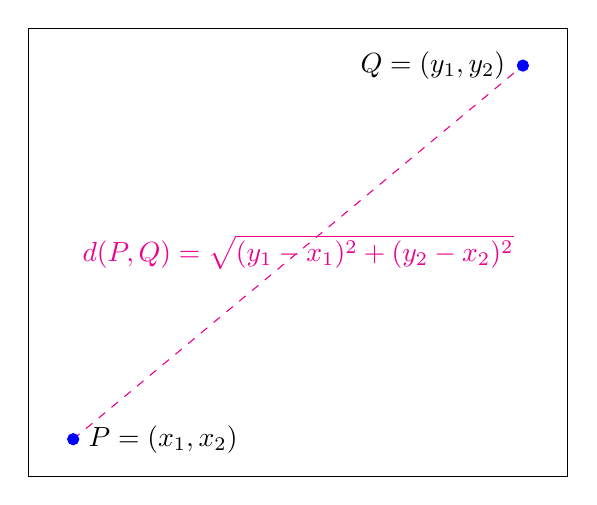
\begin{tikzpicture}
\begin{axis}[domain=0:3, xtick=\empty, ytick=\empty]
\addplot[blue, only marks] table{
1 1
2 2
};
\node[] () at (1.2,1) {\(P=(x_1,x_2)\)};
\node[] () at (1.8,2) {\(Q=(y_1,y_2)\)};
\draw[dashed, magenta] (1,1) -- (2,2)
node[midway]{\(d(P,Q)=\sqrt{(y_1-x_1)^{2}+(y_2-x_2)^{2}}\)};
\end{axis}
\end{tikzpicture}
\end{center}
Note that it carries the following properties which are natural for measuring
distance:
\begin{itemize}
\item \(d(P,Q)\ge 0\) for any points \(P,Q\in\R^{2}\), and \(d(P,Q)=0\) iff \(P=Q\)
\begin{intuition} Distance should be nonnegative. Also, given a point
\(\bullet\), the only point having \emph{zero} distance from (the same
``position'' as) \(\bullet\) is the point \(\bullet\) itself.
 \end{intuition}
\item \(d(P,Q)=d(Q,P)\) for any points \(P,Q\in\R^{2}\) \begin{intuition}
Distance between \(P\) and \(Q\) = distance between \(Q\) and \(P\).
\end{intuition}
\item (\emph{triangle inequality}) \(d(P,R)\le d(P,Q)+d(Q,R)\) for any points
\(P,Q,R\in\R^{2}\).
\begin{center}
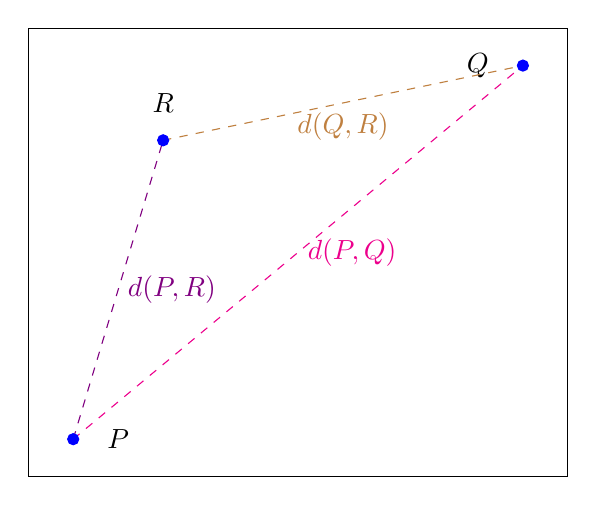
\begin{tikzpicture}
\begin{axis}[domain=0:3, xtick=\empty, ytick=\empty]
\addplot[blue, only marks] table{
1 1
2 2
1.2 1.8
};
\node[] () at (1.1,1) {\(P\)};
\node[] () at (1.9,2) {\(Q\)};
\node[] () at (1.2,1.9) {\(R\)};
\draw[dashed, magenta] (1,1) -- (2,2)
node[midway, right]{\(d(P,Q)\)};
\draw[dashed, violet] (1,1) -- (1.2,1.8)
node[midway, right]{\(d(P,R)\)};
\draw[dashed, brown] (1.2,1.8) -- (2,2)
node[midway, below]{\(d(Q,R)\)};
\end{axis}
\end{tikzpicture}
\end{center}
\end{itemize}
These properties define a \emph{metric}.
\item Let \(X\) be a nonempty set. Then, a \defn{metric} is a function
\(d:X\times X\to\R\) satisfying:
\begin{enumerate}[label={(M\arabic*)}]
\item For any \(x,y\in X\), \(d(x,y)\ge 0\) and \(d(x,y)=0\) iff \(x=y\).
\item For any \(x,y\in X\), \(d(x,y)=d(y,x)\).
\item For any \(x,y,z\in X\), \(d(x,z)\le d(x,y)+d(y,z)\).
\end{enumerate}
We also call the ordered pair \((X,d)\) a \defn{metric space}.

\begin{note}
When the choice of the metric \(d\) is clear from context, we may simply write
\(X\) instead of \((X,d)\). For example, unless stated otherwise, the metric
chosen when \(X=\R^n\) would the Euclidean distance.
\end{note}

This definition of metric space captures the idea of \emph{points} and
\emph{distances}. For any \(x,y\in X\), \(d(x,y)\) is the \defn{distance
between \(x\) and \(y\) with respect to \(d\)}. Elements in \(X\) are
\defn{points}.

\item Sometimes we only want to focus on a certain ``part'' of a metric space
(without altering the way of measuring distance). This leads to the notion of
\emph{metric subspace}. Let \((X,d)\) be a metric space and let \(Y\) be a
nonempty subset of \(X\). Define \(d_Y:Y\times  Y\to \R\) by
\[
d_Y(x,y)=d(x,y)
\]
for any \(x,y\in Y\). Then, \((Y,d_Y)\) is called a \defn{metric subspace} of
\((X,d)\) and \(d_Y\) is called as the \defn{relative metric induced by \(d\)
on \(Y\)}.

\item\label{it:metric-subspace-is-ms} In fact, \((Y,d_Y)\) is also a metric space.

\begin{pf}
Since \((X,d)\) is a metric space, (M1)--(M3) hold for all the points in \(X\).
Now, as \(Y\subseteq X\), every point in \(Y\) is also a point in \(X\), so
immediately (M1)--(M3) are satisfied for all the points in \(Y\) also.
\end{pf}
\end{enumerate}
\subsection{Examples of Metric Spaces}
\label{subsect:metric-sp-eg}
\begin{enumerate}
\item The definition of metric space is quite general. Indeed, many kinds of
sets (equipped with a certain metric \(d\)) can be metric spaces. We will give
some examples of metric spaces in \Cref{subsect:metric-sp-eg} and \emph{prove}
that some are indeed metric spaces.

\item \label{it:metric-rn}
(a familiar one) Let \(X=\R^n\). For any points \(P=(x_1,\dotsc,x_n)\)
and \(Q=(y_1,\dotsc,y_n)\) in \(\R^n\), define
\(d(P,Q)=\sqrt{(y_1-x_1)^{2}+\dotsb+(y_n-x_n)^{2}}\) (Euclidean distance).
Then, \((X,d)\) is a metric space.

\begin{pf}
For (M1), \(d(P,Q)\ge 0\) follows from the nonnegativity of square root
function. Also, we have
\[
d(P,Q)=0\iff (y_1-x_1)^{2}+\dotsb+(y_n-x_n)^{2}=0
\iff \begin{cases}
y_1=x_1\\
y_2=x_2\\
\quad\;\vdots\\
y_n=x_n
\end{cases}
\iff
P=Q.
\]
(M2) follows from the property that \((y_i-x_i)^{2}=(x_i-y_i)^{2}\) for any
\(i=1,\dotsc,n\).

(M3) can be proven by using some algebraic tricks and Cauchy-Swartz inequality,
but we shall omit the details.
\end{pf}

\item Let \(X=S^2=\{(x,y,z):x^2+y^2+z^2=1\}\subseteq\R^3\), an unit sphere in
\(\R^3\).
\begin{center}
\begin{tikzpicture}
\draw[blue] (0,0) circle [radius=3cm];
\draw[blue] (-3,0) arc (180:360:3 and 0.6);
\draw[blue, dashed] (3,0) arc (0:180:3 and 0.6);
\node[violet, fill, circle, inner sep=0pt, minimum size=1.5mm] (start) at (0,-0.3) {};
\node[] () at (0.5,-0.3) {start};
\node[] () at (1.5,1.414) {end};
\node[brown, fill, circle, inner sep=0pt, minimum size=1.5mm] (end) at (1,1.414) {};
\draw[->, dashed, green!50!black] (start) .. controls (0.4, 0.25) .. (end);
\draw[->, dashed, red] (start) .. controls (-5.7,-6.95) and (3.7,5.95) .. (end);
\end{tikzpicture}
\end{center}
To motivate the definition of the following metric, suppose that the unit
sphere represents the ``Earth'' \faIcon{globe-americas}, and the two points
(\({\color{violet}\bullet}\) and \({\color{brown}\bullet}\)) on it represent
two places. Now, suppose that you want to travel \faIcon{plane} from
\({\color{violet}\bullet}\) to \({\color{brown}\bullet}\). Intuitively, the
shortest path for the travel is represented by the {\color{green!50!black}green
dashed arrows} (one cannot ``drill through the Earth straightly'' to go to
\({\color{brown}\bullet}\)!). It then appears that the arc length of that path
should be the distance between the two points.

Mathematically, we define \(d(x,y)=\) the length of the smaller arc on the
unique great circle (a planar circle on \(S^2\) with unit radius) joining the
two points \(x\) and \(y\). Then, \((X,d)\) is again a metric space.

\begin{pf}
Omitted.
\end{pf}
\item It turns out that one can form a metric space from \emph{any} set, using
the \emph{discrete metric}. Let \(X\) be any set. Then, for any \(x,y\in X\),
define
\[
d(x,y)=1-\delta_{xy}
\]
where \(\displaystyle \delta_{xy}=\begin{cases}
1&\text{if \(x=y\)};\\
0&\text{otherwise}.
\end{cases}
\) This metric is called \defn{discrete metric}, under which the distance
between two different points is \emph{always} one, and the distance between two
identical points are zero. \((X,d)\) is a metric space, which is sometimes
called \defn{discrete metric space}.

\begin{pf}
Fix any \(x,y\in X\). Then, since \(d(x,y)=0\text{ or }1\), it must be
nonnegative. Furthermore, we have \(d(x,y)=0\iff \delta_{xy}=1\iff x=y\), so
(M1) is satisfied.

(M2) follows from the fact that \(\delta_{xy}\) is symmetric (i.e.,
\(\delta_{xy}=\delta_{yx}\)).

For (M3), we prove by cases.
\begin{itemize}
\item Case 1: \(x=z\). Then, we have \(d(x,z)=0\le d(x,y)+d(y,z)\) (as RHS must
be nonnegative).
\item Case 2: \(x\ne z\). Then, \(d(x,z)=1\). Now, consider:
\begin{enumerate}
\item Subcase 1: \(x\ne y\). Then, \(d(x,y)+d(y,z)=(1+0)\text{ or }(1+1)\).
\item Subcase 2: \(z\ne y\). Then, \(d(x,y)+d(y,z)=(0+1)\text{ or }(1+1)\).
\end{enumerate}
In either subcase, we have \(d(x,y)+d(y,z)\ge 1=d(x,z)\), as desired.
\end{itemize}
\end{pf}
\item As mentioned earlier, MATH3401 is about studying continuous functions on
metric space. So, here we consider an example of a metric space for a set of
\emph{continuous functions}. Let \(X=C[a,b]\), the set of all real-valued
continuous functions with domain \([a,b]\). In this case, each ``point'' is
indeed a function, rather than a number. How should we measure the
distance between two \emph{functions}?

There are multiple ways to do so, but the following three are relatively more
famous. For any functions \(f,g\in X\):
\begin{itemize}
\item \textit{\(L^2\) norm:}
\[
d_2(f,g)=\qty[\int_{a}^{b}[f(x)-g(x)]^{2}\dd{x}]^{1/2}\triangleq\|f-g\|_{2}.
\]
\item \textit{\(L^1\) norm:}
\[
d_1(f,g)=\int_{a}^{b}|f(x)-g(x)|\dd{x}\triangleq\|f-g\|_{1}.
\]
\item \textit{\(L^{\infty}\) norm:}
\[
d_{\infty}(f,g)=\sup\{|f(x)-g(x)|:x\in[a,b]\}\triangleq\|f-g\|_{\infty}.
\]
\begin{note}
In general, for any \(p\ge 1\), we have the \emph{\(L^p\) norm}:
\[
d_p(f,g)=\qty[\int_{a}^{b}[f(x)-g(x)]^{p}\dd{x}]^{1/p}\triangleq\|f-g\|_{p}.
\]
It turns out that the limit of \(d_{p}(f,g)\) as \(p\to\infty\) is
\(\sup\{|f(x)-g(x)|:x\in[a,b]\}\), hence the name ``\(L^\infty\) norm''.
\end{note}

\begin{intuition}
\(L^1\) and \(L^2\) norms capture the intuitive idea that two functions \(f\)
and \(g\) are ``close'' if for ``most'' input \(x\), \(f(x)\) and \(g(x)\) are
``close''.
\end{intuition}
\end{itemize}
\item The last example we give here concerns a metric space with \emph{finite}
set. Let \(X=\{a,b,c\}\) (where \(a\), \(b\), and \(c\) are distinct). Define
the function \(d:X\times X\to\R\) by
\begin{center}
\begin{tabular}{c|ccc}
\toprule
\(d\)&\(a\)&\(b\)&\(c\)\\
\midrule
\(a\)&0&2&3\\
\(b\)&2&0&2\\
\(c\)&3&2&0\\
\bottomrule
\end{tabular}
\end{center}
Then, \((X,d)\) is a metric space.

\begin{pf}
(M1) follows since every entry in the table is nonnegative and all the
diagonal entries are zero. (M2) follows since the table is symmetric along its
diagonal.

For (M3), we can exhaust all the possibilities (since there are only finitely
many possible pairs of points) and verify it.
\end{pf}
\end{enumerate}
\subsection{Distance Between a Point and a Set}
\label{subsect:pt-set-dist}
\begin{enumerate}
\item Apart from distance between two points, sometimes we are interested in
knowing distance between a point and a set. How should we define it?
\begin{center}
\begin{tikzpicture}
\draw[fill, blue] (0,0) circle [radius=0.5mm];
\draw[fill, magenta!20!white] (-5,0) ellipse [x radius=2cm, y radius=1cm];
\node[] (set) at (-5,0) {\(S\)};
\node[] (pt) at (0,-0.5) {\(P\)};
\draw[-Latex] (-2.5,-2) -- (set);
\draw[-Latex] (-2.5,-2) -- (pt);
\node[] () at (-2.5,-2.5) {distance?};
\end{tikzpicture}
\end{center}

\item An intuitive way to measure the distance between the point \(P\) and the
set \(S\) is to use the length of the ``\emph{shortest}'' path for ``travelling''
from point \(P\) (``your current location'') to set \(S\) (``island'').
\begin{center}
\begin{tikzpicture}
\draw[fill, magenta!20!white] (-5,0) ellipse [x radius=2cm, y radius=1cm];
\node[] (set) at (-5,0) {\(S\)};
\node[] () at (-6,0.6) {\faIcon{tree}};
\node[] () at (-6,-0.5) {\faIcon{tree}};
\node[] () at (-4.5,-0.3) {\faIcon{tree}};
\node[] () at (-5.5,0.4) {\faIcon{tree}};
\node[] (pt) at (0,-0.5) {\(P\)};
\node[] () at (0,0) {\faIcon{swimmer}};
\draw[fill, blue] (0,0) circle [radius=0.5mm];
\draw[-Latex, dashed, green!50!black] (0,0) -- (-3,0)
node[midway, above]{shortest};
\draw[-Latex, dashed, red, opacity=0.5] (0,0) -- (-3.5,-0.6614);
\draw[-Latex, dashed, red, opacity=0.5] (0,0) -- (-4,0.86603);
\end{tikzpicture}
\end{center}
\item Mathematically, in a metric space \((X,d)\), given any point \(P\in X\)
and any nonempty set \(S\subseteq X\), the \defn{distance from point \(P\) to
set \(S\)} is
\[
d(P,S)=\inf_{x\in S}d(P,x).
\]
\begin{note}
The notation \(\displaystyle \inf_{x\in S}d(P,x)\) is another way to write
\(\inf\{d(P,x):x\in S\}\). This applies to ``\(\sup\)'' similarly.
\end{note}
\item Now, after ``arriving'' the set \(S\) (``island''), we may start
``exploring'' \faIcon{search} it. We would then like to know how ``large'' the
``island'' is, which may be measured by its ``diameter''.
\begin{center}
\begin{tikzpicture}
\draw[fill, magenta!20!white] (-5,0) ellipse [x radius=2cm, y radius=1cm];
\node[] (set) at (-5,0) {\(S\)};
\node[] () at (-6,0.6) {\faIcon{tree}};
\node[] () at (-6,-0.5) {\faIcon{tree}};
\node[] () at (-4.5,-0.3) {\faIcon{tree}};
\node[] () at (-5.5,0.4) {\faIcon{tree}};
\node[] () at (-3,0) {\faIcon{child}};
\end{tikzpicture}
\end{center}
\item Recall the notion of \emph{diameter} for a circle. It is the length of a
line segment passing through the center and whose endpoints lie on the circle.
It is also the \emph{maximum distance} between two points lying on the circle.
\begin{center}
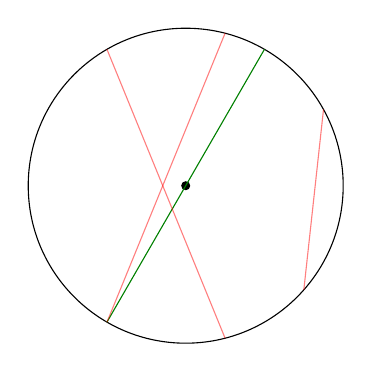
\begin{tikzpicture}
\draw[] (0,0) circle [radius=2cm];
\draw[fill] (0,0) circle [radius=0.5mm];
\draw[green!50!black] (-1,-1.732) -- (1,1.732);
\draw[red, opacity=0.5] (-1,-1.732) -- (0.5,1.936);
\draw[red, opacity=0.5] (1.5,-1.323) -- (1.75,0.9682);
\draw[red, opacity=0.5] (-1,1.732) -- (0.5,-1.936);
\end{tikzpicture}
\end{center}
In a similar manner, we may define the notion of \emph{diameter} for other
kinds of geometrical objects as follows.

Let \((X,d)\) be a metric space. For any nonempty set \(S\subseteq X\), the
\defn{diameter} of \(S\) is
\[
D(S)=\sup_{P,Q\in S}\{d(P,Q)\}.
\]
We have \(D(S)=\infty\) when the set \(\{d(P,Q):P,Q\in S\}\) is not bounded
above. For convenience, we extend the notion of \emph{diameter} to an empty
set by defining \(D(\varnothing)=-\infty\).

\item The set \(S\) is said to be \defn{bounded} if \(D(S)\ne\infty\) (equivalently,
\(\{d(P,Q):P,Q\in S\}\) is bounded above, or there exists \(M>0\) such that
\(d(P,Q)\le M\) for any \(P,Q\in S\)). A function from any non-empty set to \(X\)
is said to be \defn{bounded} if its range is bounded.

\item Examples: Consider the metric space \(\R\) (equipped with Euclidean
distance). Then:
\begin{itemize}
\item the diameter of the closed interval \([0,1]\) is \(1\)
\item the diameter of the open interval \((0,1)\) is \(1\) \begin{note}
If we use ``\(\max\)'' instead of ``\(\sup\)'' in the definition for diameter,
then this is \emph{undefined}, which is unsatisfactory. Hence, in the
definition we use the notion of supremum instead of maximum.
\end{note}
\end{itemize}
\end{enumerate}
\subsection{Topology of Metric Spaces}
\label{subsect:metric-spaces-topo}
\begin{enumerate}
\item Roughly speaking, \emph{topology} studies the properties of a geometric
object that are preserved under ``continuous deformations''. Here, we will
introduce some important notions related to metric space topology.

\item For the case of \(\R\), we are familiar with the notions of \emph{open
interval} (interval not including its endpoints) and \emph{closed interval}
(interval including its endpoints). We can generalize these notions to
\emph{open sets} and \emph{closed sets} respectively, which are fundamental to
metric space topology.

\item To define open and closed sets, we need to introduce some preliminary
notions. Consider a metric space \((X,d)\) throughout. Let \(a\in X\) and
\(r>0\). Then, the \defn{open ball} in \(X\) with center \(a\) and radius \(r\)
is
\[
B(a,r)=\{x\in X: d(a,x)\vc{<}r\},
\]
and the \defn{closed ball} in \(X\) with center \(a\) and radius \(r\) is
\[
\overline{B}(a,r)=\{x\in X: d(a,x)\vc{\le}r\},
\]
\begin{center}
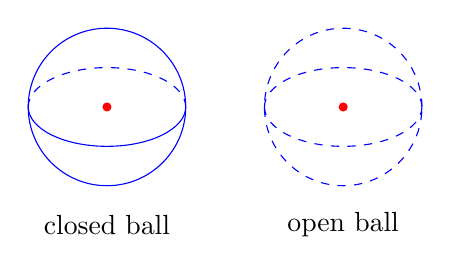
\begin{tikzpicture}
\draw[blue] (0,0) circle [radius=1cm];
\draw[blue] (-1,0) arc (180:360:1 and 0.5);
\draw[blue, dashed] (1,0) arc (0:180:1 and 0.5);
\draw[red, fill] (0,0) circle [radius=0.5mm];
\node[] () at (0,-1.5) {closed ball};

\draw[blue, dashed] (3,0) circle [radius=1cm];
\draw[blue, dashed] (2,0) arc (180:360:1 and 0.5);
\draw[blue, dashed] (4,0) arc (0:180:1 and 0.5);
\draw[red, fill] (3,0) circle [radius=0.5mm];
\node[] () at (3,-1.5) {open ball};
\end{tikzpicture}
\end{center}
\begin{note}
Let \(S\) be a nonempty subset of \(X\).  Considering \((S,d)\) as a metric
subspace of \((X,d)\) (which is itself a metric space), an open ball in \(S\)
with center \(a\) and radius \(r\) can be expressed as
\[
B_{S}(a,r)=\{x\in S:d(a,x)<r\}=B_{X}(a,r)\cap S
\]
where \(B_X(a,r)\) is the open ball with same center and radius, but in \(X\).
\end{note}
\item Let \(S\subseteq X\). Then, a point \(a\in S\) is an \defn{interior
point} of \(S\) if there exists \(r>0\) such that \[
B(a,r)\subseteq S.
\]
The \defn{interior} of \(S\), denoted by \defn{\(S^{\circ}\)} or
\defn{\(\operatorname{int}S\)}, is the set of all interior points of \(S\).

\begin{intuition}
Viewing \(S\) as an ``island'', an interior point of \(S\) is a location at the
``inner part'' of ``island'', and the interior of \(S\) is the whole ``inner
part'' of ``island''.
\end{intuition}

\begin{center}
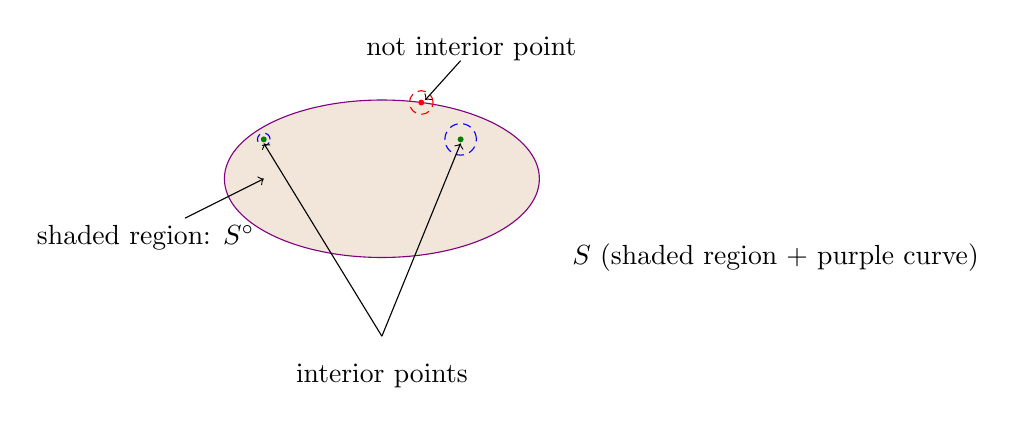
\begin{tikzpicture}
\draw[fill, brown!20!white, draw=violet] (0,0) ellipse [x radius=2cm, y radius=1cm];
\draw[fill, green!50!black] (1,0.5) circle [radius=0.3mm];
\draw[draw, densely dashed, blue] (1,0.5) circle [radius=2mm];
\draw[fill, green!50!black] (-1.5,0.5) circle [radius=0.3mm];
\draw[draw, densely dashed, blue] (-1.5,0.5) circle [radius=0.8mm];
\draw[fill, red] (0.5,0.9682) circle [radius=0.3mm];
\draw[draw, densely dashed, red] (0.5,0.9682) circle [radius=1.5mm];
\draw[->] (1,1.5) -- (0.55,1)
node[pos=-0.3]{not interior point};
\draw[->] (0,-2) -- (-1.5,0.45);
\draw[->] (0,-2) -- (1,0.45);
\node[] () at (0,-2.5) {interior points};
\node[] () at (5,-1) {\(S\) (shaded region + purple curve)};
\draw[->] (-2.5,-0.5) -- (-1.5,0)
node[pos=-0.5]{shaded region: \(S^{\circ}\)};
\end{tikzpicture}
\end{center}

\item Now we are ready to define open and closed sets. A set \(S\subseteq X\)
is \defn{open} in \(X\) if \(S=S^{\circ}\), and it is \defn{closed} in \(X\) if
\(X\setminus S\) is open in \(X\).
\begin{center}
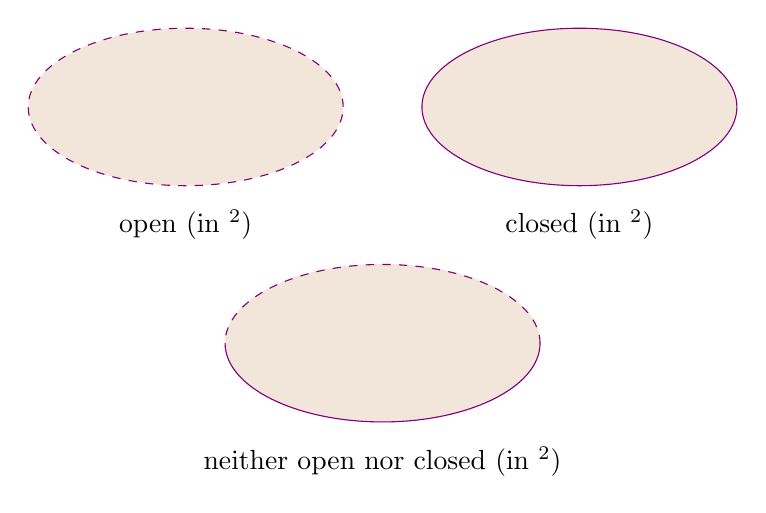
\begin{tikzpicture}
\draw[fill, brown!20!white, draw=violet, dashed] (0,0) ellipse [x radius=2cm, y radius=1cm];
\node[] () at (0,-1.5) {open (in \(\R^2\))};
\draw[fill, brown!20!white, draw=violet] (5,0) ellipse [x radius=2cm, y radius=1cm];
\node[] () at (5,-1.5) {closed (in \(\R^2\))};
\draw[fill, brown!20!white] (2.5,-3) ellipse [x radius=2cm, y radius=1cm];
\draw[violet, dashed] (4.5,-3) arc (0:180:2 and 1);
\draw[violet] (0.5,-3) arc (180:360:2 and 1);
\node[] () at (2.5,-4.5) {neither open nor closed (in \(\R^2\))};
\end{tikzpicture}
\end{center}
\begin{remark}
\item For convenience in wordings, sometimes we write ``\(S\) is an open
(closed) subset/set of \(X\)'' or ``\(S\) is an open (closed) set in \(X\)''
to mean that \(S\subseteq X\) is open (closed) in \(X\).

\item When the set \(S\) is empty, there is no interior point of \(S\) (since \(S\)
does not even have element!). Thus, the interior of \(S\) is empty as well.
Hence, we have \(S=S^{\circ}=\varnothing\), meaning that empty set is open in
\(X\). (This holds true for any metric space \((X,d)\)!)

\item The concepts of ``open'' and ``closed'' are with respect to the metric
space \((X,d)\). So, we should specify what metric space \((X,d)\) we are
referring to when talking about open and closed sets, unless it is clear from
context.
\end{remark}
\item \label{it:openness-equiv-def}
We always have \(S\supseteq S^{\circ}\) since every interior point of
\(S\) must be an element of \(S\) (by definition). Hence, to show that a set
\(S\) is open in \(X\), it suffices to show that \(S\subseteq S^{\circ}\),
i.e., every point in \(S\) is an interior point of \(S\).

More explicitly, this means that \(S\) is open in \(X\) iff for any \(x\in S\),
there exists \(r>0\) such that \(B(x,r)\subseteq S\). This may serve as a
definition of openness that is more convenient to be checked.

\item The concepts of open and closed sets are not mutually exclusive. Indeed,
a set can be \emph{both open and closed}.
\begin{proposition}
\label{prp:both-open-and-closed}
Let \((X,d)\) be a metric space. Then, \(\varnothing\) and \(X\) are both open
and closed in \(X\).
\end{proposition}
\begin{pf}
Firstly, from the remark above we know that \(\varnothing\) is open in \(X\).
Now we will show that \(X\) is also open in \(X\). Consider any point \(a\in
X\), and choose any \(r>0\). Then, we immediately have
\[
B(a,r)=\{x\vc{\in X}:d(a,x)<r\}\vc{\subseteq X},
\]
meaning that the point \(a\) is an interior point of \(X\). Thus, we have
\(X\subseteq X^{\circ}\) (which implies that \(X=X^{\circ}\)) and hence \(X\)
is open in \(X\).

Next, note that \(\varnothing=X\setminus \blc{X}\) and
\(X=X\setminus\brc{\varnothing}\) are open in \(X\). Thus, \(\blc{X}\) and
\(\brc{\varnothing}\) are closed in \(X\).
\end{pf}

\item For different metric spaces, the same set can have different properties
regarding openness and closedness. The following example illustrates this
phenomenon.

Let \(X=\R\) and equip it with the Euclidean distance metric \(d\) (defined by
\(d(x,y)=|x-y|\) for any \(x,y\in X\)). Let \(Y=[0,1)\cup (2,3)\subseteq X\),
which induces a metric subspace of \((X,d)\): \((Y,d_{Y}\)). Then, \(S=[0,1)\)
is neither open nor closed in \(X\), but is both open and closed in \(Y\).

\begin{pf}
Firstly, \(S=[0,1)\) is not open in \(X\) since \(0\in S\) is \emph{not} an
interior point of \(S\) (for any \(r>0\), the open ball \(B(0,r)\) contains
elements outside \(S\)). It is also not closed in \(X\) since \(X\setminus
S=(-\infty,0)\cup[1,\infty)\) is not open in \(X\) (we can similarly show that
\(1\) is not an interior point of \(X\setminus S\)). This shows \(S\) is
neither open nor closed in \(X\).
\begin{center}
\begin{tikzpicture}
\draw[-Latex] (0,0) -- (10,0);
\node[] () at (3,0) {[};
\node[] () at (7,0) {)};
\node[] () at (3,-0.5) {\(0\)};
\node[] () at (7,-0.5) {\(1\)};
\node[blue] () at (2.8,0) {(};
\node[blue] () at (3.2,0) {)};
\draw[line width=0.1cm, opacity=0.5, red, line cap=round] (2.8,0) -- (2.93,0);
\draw[red, ->] (2,-1) -- (2.85,-0.2)
node[pos=-0.3]{outside \(S\)!};
\end{tikzpicture}
\end{center}

Next, we will prove that \(S\) is both open and closed in \(Y\). For the
openness, we will only show that \(0\) is an interior point of \(Y\). (Every
other point in \(S\) is clearly an interior point of \(Y\), by choosing
a sufficiently small \(r>0\) (e.g., \(\displaystyle
r=\frac{1}{2}\cdot \max\{\text{distance between the point and \(0\)}, \text{distance
between the point and \(1\)}\}\)).)

We first need to choose a small \(r>0\), say \(r=0.1\). Then, we have
\[
B(0,r)=\{y\in\vc{Y}:|y-0|<r\}
=\{y\in\vc{[0, 1)\cup (2,3)}:y<0.1\}
=[0,0.1)\subseteq Y
\]
(which is \underline{not} \((-0.1,0.1)\) \warn{}). Thus, \(0\) is an interior
point of \(Y\), and hence \(S\) is open in \(Y\).
\begin{center}
\begin{tikzpicture}
\draw[-Latex] (0,0) -- (10,0);
\node[] () at (3,0) {[};
\node[] () at (7,0) {)};
\node[] () at (3,-0.5) {\(0\)};
\node[] () at (7,-0.5) {\(1\)};
\node[blue] () at (3,0) {[};
\node[blue] () at (3.2,0) {)};
\draw[violet, ->] (3.5,-1) -- (3.1,-0.2)
node[pos=-0.3]{altered ``shape'' of \(B(0,r)\)};
\end{tikzpicture}
\end{center}
For the closedness, note that \(Y\setminus S=(2,3)\). Every point in
\(Y\setminus S\) can be shown to be an interior point of \(Y\) (by choosing a
sufficient small \(r>0\), like what was mentioned above). So, \(Y\setminus S\)
is open in \(Y\), thus \(S\) is closed in \(Y\).
\end{pf}

\item Next, we will show that any open (closed) ball in \(X\) is open (closed)
in \(X\), as suggested by its name. It turns out that it is not that trivial to
prove this!

\item \label{it:open-ball-open}
For any \(a\in X\) and \(r>0\), the open ball \(S=B(a,r)\) is open in
\(X\).

\begin{pf}
For any \(x\in S\), let \(r_0=d(x,a)\), which is less than \(r\) by the
definition of open ball. Now, choose \(\displaystyle r_1=\frac{r-r_0}{2}\).
Then, for any \(y\in B(x,r_1)\), we have
\[
d(y,a)\le \underbrace{d(y, x)}_{<r_1}+\underbrace{d(x, a)}_{r_0}
<\frac{r-r_0}{2}+r_0
=\frac{r+r_0}{2}<r\quad\text{(as \(r_0<r\))},
\]
thus \(y\in S=B(a,r)\). This means that \(B(x,r_1)\subseteq S\), i.e., \(x\) is
an interior point of \(S\). Since \(x\) is arbitrary, it follows that every
point in \(S\) is an interior point of \(S\), so \(S\) is open in \(X\).
\end{pf}
\begin{center}
\begin{tikzpicture}
\draw[violet, dashed] (0,0) circle [radius=2cm];
\draw[fill, green!50!black] (1,0.5) circle [radius=0.3mm];
\draw[fill, orange] (0,0) circle [radius=0.3mm];
\draw[draw, densely dashed, blue] (1,0.5) circle [radius=5mm];
\draw[very thick, decorate,decoration={mirror, calligraphic brace, amplitude=5pt, raise=5pt}] (0,0) -- (1.789,0.894);
\node[] () at (1,-0.2) {\(r\)};
\draw[very thick, decorate,decoration={calligraphic brace, amplitude=5pt, raise=5pt}] (0,0) -- (1,0.5);
\node[] () at (0.3,1) {\(r_0\)};
\draw[magenta, very thick, decorate,decoration={brace, amplitude=5pt, raise=5pt}] (1,0.5) -- (1.447,0.724);
\node[] () at (1.2,1.2) {\(\frac{r-r_0}{2}\)};
\end{tikzpicture}
\end{center}

\item \label{it:closed-ball-closed}
For any \(a\in X\) and \(r>0\), the closed ball \(S=\overline{B}(a,r)\)
is closed in \(X\).

\begin{pf}
Firstly, if \(S=X\), there is nothing to prove (we know that \(X\) is both open
and closed in \(X\)). Thus henceforth we will assume that
\(S=\overline{B}(x,r)\) is a proper subset of \(X\) (we know that it is a
subset of \(X\), by definition). Then, \(X\setminus S\) is nonempty.

Now, for any \(x\in X\setminus S=X\setminus\overline{B}(a,r)\), we let
\(r_0=d(x,a)>r\). Now, choose \(\displaystyle r_1=\frac{r_0-r}{2}\). Then, for
any \(y\in B(x, r_1)\), rearranging the inequality in (M3) gives
\[
d(y,a)\ge \underbrace{d(x,a)}_{r_0}-\underbrace{d(x,y)}_{<r_1}
>r_0-\frac{r_0-r}{2}
=\frac{r_0+r}{2}>r.
\]
This implies that \(y\notin\overline{B}(a,r)\), and hence \(y\in
X\setminus\overline{B}(a,r)\). Thus, we have
\[
B(x,r_1)\subseteq X\setminus S=X\setminus\overline{B}(a,r),
\]
which means that \(X\setminus S\) is open in \(X\), and so \(S\) is closed in
\(X\).
\end{pf}
\begin{center}
\begin{tikzpicture}
\draw[violet] (0,0) circle [radius=2cm];
\draw[fill, orange] (0,0) circle [radius=0.3mm];
\draw[fill, green!50!black] (3,1.5) circle [radius=0.3mm];
\draw[draw, densely dashed, blue] (3,1.5) circle [radius=5mm];
\draw[very thick, decorate,decoration={mirror, calligraphic brace, amplitude=5pt, raise=5pt}] (0,0) -- (1.789,0.894);
\node[] () at (1,-0.2) {\(r\)};
\draw[very thick, decorate,decoration={calligraphic brace, amplitude=5pt, raise=5pt}] (0,0) -- (3,1.5);
\node[] () at (1.3,1.3) {\(r_0\)};
\draw[magenta, very thick, decorate,decoration={mirror, brace, amplitude=5pt, raise=5pt}] (2.552,1.276) -- (3,1.5);
\node[] () at (3.2,0.6) {\(\frac{r_0-r}{2}\)};
\end{tikzpicture}
\end{center}

\item Apart from \emph{open ball}, we also have the notion of \emph{open
neighborhood}. Consider a metric space \((X,d)\). Let \(S\) be a nonempty
subset of \(X\) and \(a\in S\). Then, an \defn{open neighborhood} of \(a\) in
\(S\) is a set \(U\subseteq S\) which contains \(a\) and is open in \(X\).
\begin{center}
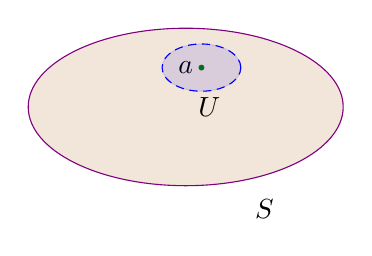
\begin{tikzpicture}
\draw[fill, brown!20!white, draw=violet] (0,0) ellipse [x radius=2cm, y radius=1cm];
\draw[fill, green!50!black] (0.2,0.5) circle [radius=0.3mm];
\node[] () at (0,0.5) {\(a\)};
\draw[draw, densely dashed, blue] (0.2,0.5) ellipse [x radius=5mm, y radius=3mm];
\draw[fill, blue, opacity=0.1] (0.2,0.5) ellipse [x radius=5mm, y radius=3mm];
\node[] () at (0.3,0) {\(U\)};
\node[] () at (1,-1.3) {\(S\)};
\end{tikzpicture}
\end{center}
More generally, a \defn{neighborhood} of \(a\) in \(S\) is a set \(U\subseteq
S\) which contains \(a\) in its interior (in \(S\)).
\begin{center}
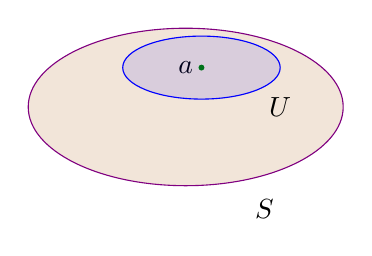
\begin{tikzpicture}
\draw[fill, brown!20!white, draw=violet] (0,0) ellipse [x radius=2cm, y radius=1cm];
\draw[fill, green!50!black] (0.2,0.5) circle [radius=0.3mm];
\node[] () at (0,0.5) {\(a\)};
\draw[draw, blue] (0.2,0.5) ellipse [x radius=1cm, y radius=0.4cm];
\draw[fill, blue, opacity=0.1] (0.2,0.5) ellipse [x radius=1cm, y radius=0.4cm];
\node[] () at (1.2,0) {\(U\)};
\node[] () at (1,-1.3) {\(S\)};
\end{tikzpicture}
\end{center}
\begin{center}
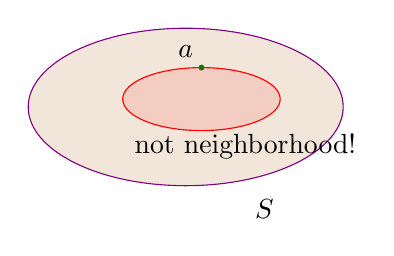
\begin{tikzpicture}
\draw[fill, brown!20!white, draw=violet] (0,0) ellipse [x radius=2cm, y radius=1cm];
\draw[fill, green!50!black] (0.2,0.5) circle [radius=0.3mm];
\node[] () at (0,0.7) {\(a\)};
\draw[draw, red] (0.2,0.1) ellipse [x radius=1cm, y radius=0.4cm];
\draw[fill, red, opacity=0.1] (0.2,0.1) ellipse [x radius=1cm, y radius=0.4cm];
\node[] () at (0.7,-0.5) {\warn{} not neighborhood!};
\node[] () at (1,-1.3) {\(S\)};
\end{tikzpicture}
\end{center}

\end{enumerate}
\subsection{Properties for Open and Closed Sets}
\begin{enumerate}
\item Here, we introduce several results that tell us some properties for the
openness and closedness.
\item The first one is about an criterion for showing that a set
\(S\) is open, which is somewhat ``similar'' to \(S\subseteq S^{\circ}\).
\begin{proposition}
\label{prp:open-set-exist-open-ball}
Let \((X,d)\) be a metric space. A set \(S\subseteq X\) is open in \(X\) iff
for any \(x\in S\), there exists an open ball (in \(X\)) \(B\) (\emph{not
necessarily centered at \(x\)}) such that \(x\in B\subseteq S\).

\begin{note}
Compare this with the condition that utilizes \(S\subseteq S^{\circ}\): A set
\(S\subseteq X\) is open in \(X\) if for any \(x\in S\), there exists \(r>0\)
such that \(B(x,r)\subseteq S\) (the open ball is necessarily centered at \(x\)).
\end{note}

\begin{pf}
``\(\Rightarrow\)'': Immediate by choosing \(B=B(x,r)\) where the latter is the
open ball \(B(x,r)\) mentioned in the note above.

``\(\Leftarrow\)'': 
\begin{center}
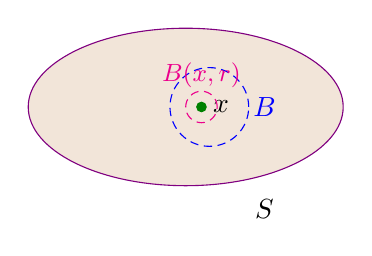
\begin{tikzpicture}
\draw[fill, brown!20!white, draw=violet] (0,0) ellipse [x radius=2cm, y radius=1cm];
\draw[fill, green!50!black] (0.2,0) circle [radius=0.6mm];
\node[] () at (0.45,0) {\(x\)};
\draw[draw, densely dashed, blue] (0.3,0) circle [radius=5mm];
\draw[draw, densely dashed, magenta] (0.2,0) circle [radius=2mm];
\node[blue] () at (1,0) {\(B\)};
\node[magenta, font=\small] () at (0.2,0.4) {\(B(x,r)\)};
\node[] () at (1,-1.3) {\(S\)};
\end{tikzpicture}
\end{center}
Assume that for any \(x\in S\), we have such open ball \(B\) where \(x\in
B\subseteq S\). Then, we can always choose a sufficiently small \(r>0\) that
makes \(B(x,r)\subseteq B\subseteq S\) (see figure above). It follows that
\(S\) is open in \(X\).
\end{pf}
\end{proposition}

\item Next, we consider the openness/closedness of union/intersection of
open/closed sets. First, we consider open sets.
\begin{proposition}
Let \((X,d)\) be a metric space.
\begin{enumerate}
\item \label{it:open-sets-union-open} The union of \emph{any collection} of open sets in \(X\) is open in \(X\).
\item \label{it:open-sets-intersect-open} The intersection of \emph{finitely
many} (\warn{} finitely many only!) open sets in \(X\) is open in \(X\).
\end{enumerate}
\end{proposition}
\begin{pf}
\begin{enumerate}
\item We write \(\displaystyle S=\bigcup_{\lambda\in\Lambda}S_{\lambda}\) where
\(S_{\lambda}\) is open in \(X\) (for any \(\lambda\in\Lambda\)), and
\(\Lambda\) is any index set. Then, we want to show that \(S\) is open in \(X\)
also. Consider any \(a\in S\). Note that \(a\in S_{\lambda^{*}}\) for some
\(\lambda^{*}\in\Lambda\) by definition. Thus, by the openness of \(S_{\lambda^{*}}\),
there exists \(r>0\) such that
\[
B(a,r)\subseteq S_{\lambda^{*}}\subseteq S.
\]
Since \(a\) is arbitrary, this implies that \(S\) is open in \(X\).

\item We write \(\displaystyle S=\bigcap_{i=1}^{n}S_i\) where \(S_{i}\) is open
in \(X\) for any \(i=1,\dotsc,n\). Then, we want to show that \(S\) is open in
\(X\).  Consider any \(a\in S\). By definition, \(a\in S_i\) for any
\(i=1,\dotsc,n\), and so by the openness there exist \(r_1,\dotsc,r_n>0\) such
that \(B(a,r_i)\subseteq S_i\) for any \(i=1,\dotsc,n\).

Now, let \(r=\min\{r_1,\dotsc,r_n\}>0\), and then we have
\[
B(a,r)\subseteq B(a,r_i)\subseteq S_i
\]
for any \(i=1,\dotsc,n\). Thus, \(B(a,r)\subseteq S\). Since \(a\) is
arbitrary, this implies that \(S\) is open in \(X\).
\end{enumerate}
\end{pf}

\item After establishing the results for open sets, we can derive the following
results for closed sets.
\begin{corollary}
Let \((X,d)\) be a metric space.
\begin{enumerate}
\item \label{it:closed-sets-union-closed}
The union of \emph{finitely many} (\warn{} finitely many only!) closed
sets in \(X\) is closed in \(X\).
\item \label{it:closed-sets-intersect-closed}
The intersection of \emph{any collection} of closed sets in \(X\) is
closed in \(X\).
\end{enumerate}
\end{corollary}
\begin{pf}
\begin{enumerate}
\item Let \(E_1,\dotsc,E_n\) be closed subsets of \(X\).
Then, \(X\setminus E_1,\dotsc,X\setminus E_n\) are all open sets in \(X\).
Thus, by \labelcref{it:open-sets-intersect-open}, the set
\[
\bigcap_{i=1}^{n}(X\setminus E_i)=X\setminus\qty(\bigcup_{i=1}^{n}E_i)\quad\text{(De Morgan's law)}
\]
is open in \(X\), so \(\displaystyle \bigcup_{i=1}^{n}E_i\) is closed in \(X\),
as desired.

\item Fix any index set \(\Lambda\), and let \(E_\lambda\subseteq X\) be a
closed set in \(X\) for any \(\lambda\in\Lambda\). Then, for any
\(\lambda\in\Lambda\),  \(X\setminus E_{\lambda}\) is open in \(X\).
Thus, by \labelcref{it:open-sets-union-open}, the set
\[
\bigcup_{\lambda\in\Lambda}(X\setminus E_{\lambda})=X\setminus\qty(\bigcap_{\lambda\in\Lambda}E_{\lambda})\quad\text{(De Morgan's law)}
\]
is open in \(X\), so \(\displaystyle \bigcap_{\lambda\in\Lambda}E_{\lambda}\) is closed in \(X\),
as desired.
\end{enumerate}
\end{pf}
\item \label{it:open-closed-equiv-crit-metric-subspace} Now, we consider again the concept of \emph{metric subspace}. Let
\((X,d)\) be a metric space. For any nonempty \(S\subseteq X\), it induces a
metric space \((S,d_S)\) (metric subspace of \((X,d)\)). We are then interested
in investigating the relationship between openness/closedness \emph{in \(S\)}
and openness/closedness \emph{in \(X\)}. We have the following relations:
\begin{enumerate}
\item \(T\subseteq S\) is open in \(S\) iff \(T=U\cap S\) for some \(U\subseteq
X\) which is open in \(X\).

\begin{pf}
``\(\Rightarrow\)'': Assume that \(T\subseteq S\) is open in \(S\). Then, for
any \(x\in T\), we can choose \(r_x>0\) such that \(B_S(x,r_x)\subseteq T\).
This implies that
\[
\bigcup_{x\in T}B_S(x, r_x)\subseteq T.
\]

Now, let \(\displaystyle U=\bigcup_{x\in T}B_X(x,r_x)\), which is open
in \(X\) by \labelcref{it:open-sets-union-open} (as the open ball
\(B_X(x,r_x)\) is always open in \(X\)).

Since \(\{x\}\subseteq B_S(x,r_x)\), we have
\[
T=\bigcup_{x\in T}\{x\}\subseteq \bigcup_{x\in T}B_S(x, r_x)\subseteq T,
\]
which forces
\[
T=\bigcup_{x\in T}B_S(x, r_x).
\]
Since \(B_S(x,r_x)=\{y\in S:d(y,x)<r_x\}=\{y\in X:d(y,x)<r_x\}\cap
S=B_X(x,r_x)\cap S\) (as \(S\subseteq X\)), by distributivity we have
\[
T=\qty(\bigcup_{x\in T}B_X(x,r_x))\cap S=U\cap S,
\]
as desired.

``\(\Leftarrow\)'': Assume that \(T=U\cap S\) for some \(U\subseteq X\) which
is open in \(X\). Then, for any \(x\in T\) (and hence \(x\in U\)), by the
openness of \(U\) there exists \(r_x>0\) such that \(B_X(x,r_x)\subseteq U\).
Thus,
\[
B_S(x,r_x)=B_X(x,r_x)\cap S\subseteq U\cap S=T,
\]
and so \(x\) is an interior point of \(T\). Since \(x\) is arbitrary, \(T\) is
open in \(S\).
\end{pf}
\item \(T\subseteq S\) is closed in \(S\) iff \(T=E\cap S\) for some
\(E\subseteq X\) which is closed in \(X\).

\begin{pf}
\begin{align*}
&\text{\(T\subseteq S\) is closed in \(S\)}\\
\iff &\text{\(S\setminus T\) is open in \(S\)}\\
\iff &\text{\(S\setminus T=U\cap S\) where \(U\subseteq X\) is open in \(X\)}\\
\iff &T=S\setminus(S\setminus T)\\
&\hspace{0.25cm}=S\setminus(U\cap S)\\
&\hspace{0.25cm}=(X\cap S)\setminus(U\cap S)&\text{(since \(S\subseteq X\))}\\
&\hspace{0.25cm}=(X\setminus U)\cap S\\
&\hspace{0.25cm}=E\cap S&\text{(\(E\subseteq X\) is closed in \(X\))}.
\end{align*}
\end{pf}
\end{enumerate}

\item Here we consider a result regarding relative complement:
\begin{proposition}
\label{prp:open-closed-comple}
Let \((X,d)\) be a metric space.  Let \(U\subseteq X\) and \(E\subseteq X\) be
open and closed sets in \(X\) respectively. Then, \(U\setminus E\) is open in
\(X\) and \(E\setminus U\) is closed in \(X\).
\end{proposition}
\begin{pf}
Firstly, \(X\setminus E\) is open in \(X\). Thus, by
\labelcref{it:open-sets-intersect-open},
\[
U\cap (X\setminus E)=U\setminus E\quad\text{(as \(U\subseteq X\))}
\]
is open in \(X\). On the other hand, note that \(X\setminus U\) is closed in
\(X\) (as \(X\setminus (X\setminus U)=U\) is open in \(X\)). Hence, by
\labelcref{it:closed-sets-intersect-closed},
\[
E\cap (X\setminus U)=E\setminus U\quad\text{(as \(E\subseteq X\))}
\]
is closed in \(X\).
\end{pf}
\item The following result connects \emph{open set} and \emph{union of open
balls}.
\begin{proposition}
\label{prp:open-set-union-open-balls}
Let \((X,d)\) be a metric space, and \(U\subseteq X\) be a nonempty set. Then,
\(U\) is open in \(X\) iff \(U\) is a union of open balls.
\end{proposition}
\begin{pf}
``\(\Rightarrow\)'': Assume that \(U\) is open in \(X\). Then for any \(x\in
U\), there exists an open ball \(B(x,r_x)\) such that \(x\in B(x,r_x)\subseteq
U\). Hence, we have
\[
U=\bigcup_{x\in U}\{x\}\subseteq \bigcup_{x\in U}B(x,r_x)\subseteq U,
\]
which forces 
\[
U=\bigcup_{x\in U}B(x,r_x),
\]
being a union of open balls.

``\(\Leftarrow\)'': Assume that \(U\) is a union of open balls. Then, we can
write
\[
U=\bigcup_{\lambda\in \Lambda}B_{\lambda}
\]
where \(B_{\lambda}\) is an open ball in \(X\) (which is also open in \(X\))
for any \(\lambda\in\Lambda\), for some index set \(\Lambda\). Thus, by
\labelcref{it:open-sets-union-open}, \(U\) is open in \(X\).
\end{pf}

\item The next result is a rather remarkable one, which is called
\emph{Lindel\"{o}f's theorem} (or \emph{Lindel\"{o}f's lemma}).
\begin{theorem}[Lindel\"{o}f's theorem]
\label{thm:lindelof}
Let \(U\subseteq \R^n\) be an open set (open in \(\R^n\)). Write
\[
U=\bigcup_{\lambda\in\Lambda}U_{\lambda}
\]
where \(\Lambda\) is an index set, and \(U_\lambda\) is open in \(\R^n\) for
any \(\lambda\in\Lambda\).  Then, there is a \emph{countable subset}
\(\{U_i:i\in\Gamma\}\subseteq \{U_{\lambda}:\lambda\in\Lambda\}\) such that
\[
U=\bigcup_{i\in\Gamma}U_{i}
\]
where \(\Gamma\) is a countable (finite or countably infinite) set of
indices.
\end{theorem}
\begin{intuition}
This result tells us that in \(\R^n\) we can always ``simplify'' an arbitrary
union of open sets to a \emph{countable} union of open sets.
\end{intuition}

\begin{pf}
Note first that the family (or set)
\[
\mathcal{U}=\qty{B\qty(q,\frac{1}{k}):q\in \Q^n, k\in\N}
\]
is countable.

Then, fix any \(x\in U\subseteq \R^n\). Since we have \(\displaystyle
U=\bigcup_{\lambda\in\Lambda}U_{\lambda}\), there exists
\(\lambda\in\Lambda\) such that \(x\in U_{\lambda}\). Furthermore,
since this \(U_{\lambda}\) is open in \(\R^n\), (by Archimedean property)
there exists \(N\in\N\) such that \(\displaystyle x\in
B\qty(x,\frac{1}{N})\subseteq U_{\lambda}\).

Next, by the \emph{density} of \(\Q^n\) on \(\R^n\)\footnote{This means that,
for every \(x\in\R^n\), the following holds: For any \(\varepsilon>0\), there
exists \(q_{x}\in\Q^n\) such that \(d(x,q_{x})<\varepsilon\).}, there exists
\(q_{x}\in\Q^n\) such that \(\displaystyle d(q_{x},x)<\frac{1}{2N}\). Now
consider the open ball \(\displaystyle Q_{x}\triangleq
B\qty(q_{x},\frac{1}{2N})\in\mathcal{U}\). Firstly, since \(\displaystyle
d(q_{x},x)<\frac{1}{2N}\), we have
\[
x\in Q_{x}\qqtext{or}\{x\}\subseteq Q_{x}.
\]
Secondly, for any \(\displaystyle y\in Q_{x}\), by triangle
inequality we have
\[
d(x,y)\le d(x,q_{x})+d(q_{x},y)
<\frac{1}{2N}+\frac{1}{2N}=\frac{1}{N},
\footnote{
We have \(\displaystyle d(x,q_{x})<\frac{1}{2N}\) by
above, and \(\displaystyle d(q_{x},y)<\frac{1}{2N}\) since
\(\displaystyle y\in Q_{x}=B\qty(q_{x},\frac{1}{2N})\).
}
\]
which means \(\displaystyle y\in B\qty(x,\frac{1}{N})\).
Thus, we have
\[
Q_{x}\subseteq B\qty(x,\frac{1}{N})\subseteq U_{\lambda}.
\]

Now, collect all these \(Q_{x}\)'s into the set \(\{Q_{x}:x\in U\}\subseteq
\mathcal{U}\). Since \(\mathcal{U}\) is countable, it follows that
\(\{Q_{x}:x\in U\}\) must also be countable. For each of the (at most countably
many) \emph{distinct} open balls in the set, from the above argument we know
that it is a subset of \(U_{\lambda}\) for some \(\lambda\in\Lambda\) (i.e.,
all points in the open ball are contained in \(U_{\lambda}\)).

We are thus able to index/relabel these (at most countably many)
\(U_{\lambda}\)'s using a countable index set \(\Gamma\). Then, collect all
these relabelled \(U_{\lambda}\)'s into the (countable) set
\(\{U_{i}:i\in\Gamma\}\subseteq \{U_{\lambda}:\lambda\in\Lambda\}\). With these
notations, we can write
\[
\bigcup_{x\in U}Q_x\subseteq \bigcup_{i\in\Gamma}U_{i}.
\]
(In words, every point falling in one of the (distinct) open balls is contained
in one of the \(U_i\)'s.)

Lastly, note that
\[
U=\bigcup_{x\in U}\{x\}\subseteq \bigcup_{x\in U}Q_x
\subseteq\bigcup_{i\in\Gamma}U_i
\subseteq \bigcup_{\lambda\in\Lambda}U_{\lambda}
=U,
\]
which implies that
\[
\bigcup_{i\in\Gamma}U_i=U,
\]
as desired.
\end{pf}

\item By \Cref{prp:open-set-union-open-balls}, every open set \(U\subseteq \R^n\) is
a union of open balls:
\[
U=\bigcup_{\lambda\in\Lambda}B_{\lambda}\quad\text{(\(B_{\lambda}\) denotes an
open ball)}.
\]
Then, applying \Cref{thm:lindelof} on this suggests that \(U\) is indeed a
\emph{countable union} of open balls (we set
\(\{U_{\lambda}:\lambda\in\Lambda\}=\{B_{\lambda}:\lambda\in\Lambda\}\), which
only contains open balls). So we can actually say more about the characteristic
of an open set \(U\) when it is a subset of \(\R^n\).

\item When \(n=1\), it turns out that we can say even more about it. We first
state the following lemma that is useful for proving the main result
later on.

\begin{lemma}
\label{lma:open-int-union-int}
Let \(U\subseteq \R\) be a nonempty set which is open in \(\R\). For any \(x\in
U\), let
\[
I_x=\bigcup_{\lambda\in\Lambda_{x}}B_{\lambda}
\]
where \(B_{\lambda}=(a_{\lambda},b_{\lambda})\) (with
\(a_{\lambda},b_{\lambda}\in\R\)) and \(\displaystyle
\Lambda_{x}=\{\lambda:\text{\(B_{\lambda}\) is an open interval with \(x\in
B_{\lambda}\subseteq U\)}\}\).

Then, we have:
\begin{enumerate}
\item \(\displaystyle I_x=\qty(\inf_{\lambda\in\Lambda_{x}}\{a_{\lambda}\}
,\sup_{\lambda\in\Lambda_x}\{b_{\lambda}\})\).

\item (maximal property) \(I_x\) is the largest open interval containing \(x\)
which is a subset of \(U\). (That is, (i) \(x\in I_x\subseteq U\) and (ii) for
any open interval \(J\) with \(x\in J\subseteq U\), \(J\subseteq
I_x\).)\footnote{Such open interval must also be unique, since when there are
two such intervals \(I\) and \(J\), we would have \(J\subseteq I\) (by the
``largest'' property of \(I\)) and \(I\subseteq J\) (by the ``largest''
property of \(J\)), which implies that \(I=J\).}

\item For any \(x,y\in U\), either \(I_x\cap I_y=\varnothing\)
(i.e., \(I_x\) and \(I_y\) are disjoint) or \(I_x=I_y\).
\end{enumerate}
\end{lemma}

\begin{pf}
\begin{enumerate}
\item ``\(\subseteq\)'': For any \(\lambda\in\Lambda_{x}\), we have
\[
\inf_{\lambda\in\Lambda_{x}}\{a_{\lambda}\}
\le a_{\lambda}\le b_{\lambda}
\le\sup_{\lambda\in\Lambda_{x}}\{b_{\lambda}\},
\]
and hence \(B_{\lambda}=(a_{\lambda},b_{\lambda})\subseteq
\qty(\inf_{\lambda\in\Lambda_{x}}\{a_{\lambda}\}
,\sup_{\lambda\in\Lambda_x}\{b_{\lambda}\})\).

Since this holds for any \(\lambda\in\Lambda_{x}\), we have
\[
I_x=\bigcup_{\lambda\in\Lambda_{x}}B_{\lambda}
\subseteq \qty(\inf_{\lambda\in\Lambda_{x}}\{a_{\lambda}\}
,\sup_{\lambda\in\Lambda_x}\{b_{\lambda}\}).
\]

``\(\supseteq\)'': For notational convenience, write \(\displaystyle
a=\inf_{\lambda\in\Lambda_{x}}\{a_{\lambda}\}\) and \(\displaystyle
b=\sup_{\lambda\in\Lambda_{x}}\{b_{\lambda}\}\). For any \(m\in(a,b)\), there
exist \(\lambda_1,\lambda_2\in\Lambda_{x}\) such that \(m>a_{\lambda_1}\) and
\(m<b_{\lambda_2}\).\footnote{First consider the case that \(a\) and \(b\)
are both finite. For the former, we utilize the result that \(\ell=\inf C\) iff
for any \(\varepsilon>0\), there exists \(c\in C\) such that
\(c<\ell+\varepsilon\). In this case, we have
\(C=\{a_{\lambda}:\lambda\in\Lambda_{x}\}\), and \(\ell=a\). Then, we set
\(\varepsilon=m-a\), and hence there exists \(\lambda_{1}\in\Lambda_{x}\) such
that \(a_{\lambda_1}<a+(m-a)=m\) (``\(a_{\lambda_1}\)'' plays the role of
``\(c\)''). The reasoning is similar for the latter.

Now, suppose \(a\) or \(b\) is not finite. Assuming \(a=-\infty\), the set
\(\{a_{\lambda}:\lambda\in\Lambda_x\}\) is not bounded below, so there always
exists \(\lambda_1\in\Lambda_x\) such that \(a_{\lambda_1}<m\) (regardless of
how small/negative \(m\) is). (The proof is similar when \(b=\infty\).)
}

Then, consider the union
\[
(a_{\lambda_1},b_{\lambda_1})\cup(a_{\lambda_2},b_{\lambda_2})
=(\min\{a_{\lambda_1},a_{\lambda_2}\},\max\{b_{\lambda_1},b_{\lambda_2}\}).
\]
Since \(a_{\lambda_1}<m<b_{\lambda_2}\), \(m\) belongs to this union.
Furthermore, since \((a_{\lambda_1},b_{\lambda_1})\) and
\((a_{\lambda_2},b_{\lambda_2})\) are both open intervals containing a common
point \(x\), their union is also an open interval containing \(x\).
\begin{center}
\begin{tikzpicture}
\draw[-Latex] (0,0) -- (10,0);
\draw[magenta, fill] (5,0) circle [radius=0.5mm];
\node[magenta] () at (5,-0.3) {\(m\)};
\node[blue] () at (3,0) {(};
\node[blue] () at (8,0) {)};
\node[blue] () at (3,-0.4) {\(a_{\lambda_1}\)};
\node[blue] () at (8,-0.4) {\(b_{\lambda_1}\)};
\node[violet] () at (1,0) {(};
\node[violet] () at (6,0) {)};
\node[violet] () at (1,-0.4) {\(a_{\lambda_2}\)};
\node[violet] () at (6,-0.4) {\(b_{\lambda_2}\)};
\draw[yellow, opacity=0.5, line width=1mm] (1,0) -- (8,0);
\end{tikzpicture}
\end{center}

Since both \((a_{\lambda_1},b_{\lambda_1})\) and
\((a_{\lambda_2},b_{\lambda_2})\) are subsets of \(U\), their union is also a
subset of \(U\). Hence, together with the result above, we know that the union
is an open interval containing \(x\) which is a subset of \(U\), so the union
can actually be expressed as \(B_{\lambda_0}\) for some
\(\lambda_0\in\Lambda_x\).

Recall that \(m\) belongs to this union, i.e., \(m\in B_{\lambda_0}\).
As \(m\) is an arbitrary element in \((a,b)\), we conclude that \(\displaystyle
(a,b)\subseteq B_{\lambda_0}\subseteq
\bigcup_{\lambda\in\Lambda_x}B_{\lambda}=I_x\).

\item It is quite straightforward to prove the maximal property. First of all,
since \(x\in B_{\lambda}\subseteq U\) for any \(\lambda\in\Lambda_{x}\), we have
\[
x\in I_x=\bigcup_{\lambda\in\Lambda_{x}}B_{\lambda}\subseteq U.
\]

Next, for any open interval \(J\) with \(x\in J\subseteq U\), it can be written
as \(B_{\lambda_J}\) for some \(\lambda_J\in\Lambda_x\). Then, we readily have
\[
B_{\lambda_{J}}\subseteq \bigcup_{\lambda\in\Lambda_x}B_{\lambda}=I_x.
\]

\item First we shall prove the following claim: For any \(x,y\in U\), if
\(\rc{y}\in I_\blc{x}\), then \(I_\blc{x}=I_{\rc{y}}\).

\begin{pf}
``\(\subseteq\)'': By (b), \(I_\rc{y}\) is the largest open interval containing
\(\rc{y}\), that is a subset of \(U\). Here, by assumption we have \(\rc{y}\in
I_\blc{x}\), and we know that \(I_\blc{x}\subseteq U\). Hence, by the maximal property of
\(I_\rc{y}\),
\[
I_\blc{x}\subseteq I_\rc{y}.
\]
``\(\supseteq\)'': Since \(I_\blc{x}\subseteq I_\rc{y}\) and \(\blc{x}\in
I_\blc{x}\), we must have \(\blc{x}\in I_\rc{y}\) (by definition of subset).
Hence, repeating the argument for ``\(\subseteq\)'' part suggests that
\[I_\rc{y}\subseteq I_\blc{x}.\]
\end{pf}

Now, to prove (c), we will prove that \(I_x\cap I_y\rc{\ne}\varnothing\implies
I_x=I_y\) (which is logically equivalent to \(I_x\cap I_y=\varnothing\) or
\(I_x=I_y\)). Assume that \(I_x\cap I_y\ne\varnothing\). Then, there exists
\(u\in I_x\cap I_y\), i.e., \(u\in I_x\) and \(u\in I_y\). By the claim above,
it implies that \(I_x=I_u\) and \(I_y=I_u\) (respectively), and thus
\(I_x=I_y\) as desired.
\end{enumerate}
\end{pf}

While the proof for \Cref{lma:open-int-union-int} is rather lengthy, it paves
the way for us to prove the following theorem more easily.
\begin{theorem}
\label{thm:union-disjoint-int}
Every nonempty open subset \(U\) of \(\R\) (open in \(\R\)) is a union of
countably many (pairwise) disjoint open intervals in \(\R\). Furthermore, such
a collection of intervals is \emph{unique}.
\end{theorem}
\begin{pf}
Consider any nonempty open subset \(U\) of \(\R\). For any \(x\in U\), let
\(\displaystyle I_x=\bigcup_{\lambda\in\Lambda_{x}}B_{\lambda}\) (which carries the same
meaning as that in \Cref{lma:open-int-union-int}).

By \Cref{lma:open-int-union-int}, we have \(I_x\cap I_y=\varnothing\) or
\(I_x=I_y\) for any \(x,y\in U\). Thus, \(\mathcal{I}=\{\text{the distinct
\(I_x\)'s}: x\in U\}\) is a collection (or set) of pairwise disjoint open
intervals whose union is \(U\) (as the collection is just essentially obtained
from removing redundancies in \(\{I_x:x\in U\}\) whose union is
\(U\)\footnote{Since \(x\in I_x\) (or \(\{x\}\subseteq I_x\)) and
\(I_x\subseteq U\) for any \(x\in U\), we have \(\displaystyle U=\bigcup_{x\in
U}\{x\}\subseteq \bigcup_{x\in U}I_x\subseteq U\).}, and removing redundancies
would not affect the outcome for the union).

Then, by Lindel\"{o}f's theorem (\Cref{thm:lindelof}), there is a \emph{countable}
sub-collection of \(\mathcal{I}\) having union equal to \(U\). But when one
removes an interval from \(\mathcal{I}\) (which is pairwise disjoint from each
of the other open intervals in \(\mathcal{I}\)), the union of the remaining
intervals in \(\mathcal{I}\) would \emph{not} be \(U\) anymore. This forces the
sub-collection to be \(\mathcal{I}\) itself. Hence, \(\mathcal{I}\)
is countable. This shows the existence part of \Cref{thm:union-disjoint-int}.

For the uniqueness part of \Cref{thm:union-disjoint-int}, suppose that there
are two such countable collections of pairwise disjoint open intervals
\(\mathcal{I}=\{I_{\gamma}:\gamma\in\Gamma\}\) and
\(\mathcal{J}=\{J_{\theta}:\theta\in\Theta\}\) (with some relabelling on the
indices), where each of the collections has a union equal to \(U\), i.e.,
\[
\bigsqcup_{\gamma\in\Gamma}I_{\gamma}=\bigsqcup_{\theta\in\Theta}J_{\theta}=U.
\]
\begin{note}
The notation \(\bigsqcup\) denotes \emph{disjoint union}, which carries the same
meaning as \(\bigcup\), but it emphasizes that the sets involved in the union
are pairwise disjoint.
\end{note}
Due the pairwise disjoint property, for any \(x\in U\), there exists a
\emph{unique} \(I_{\gamma_x}\) and a \emph{unique} \(J_{\theta_x}\) (in
\(\mathcal{I}\) and \(\mathcal{J}\) respectively) such that \(x\in I_{\gamma_x}\)
and \(x\in J_{\theta_x}\). This implies that \(I_{\gamma_x}=I_x=J_{\theta_x}\) (see
the claim in the proof of \Cref{lma:open-int-union-int}).

As we consider all \(x\in U\), the equality would ``involve'' all pairs of
intervals in \(\mathcal{I}\) and \(\mathcal{J}\), and so we conclude that
\(\mathcal{I}=\mathcal{J}\), establishing the uniqueness.
\end{pf}
\end{enumerate}
\subsection{Adherent, Accumulation, and Boundary Points}
\label{subsect:adher-accum-bound-pts}
\begin{enumerate}
\item We have introduced the notion of \emph{openness} and \emph{closedness} in
\Cref{subsect:metric-spaces-topo}, which describe \emph{sets}. In
\Cref{subsect:adher-accum-bound-pts}, we will introduce some notions that
describe \emph{points} (in addition to \emph{interior points} in
\Cref{subsect:metric-spaces-topo}). Throughout
\Cref{subsect:adher-accum-bound-pts}, we shall work in a metric space
\((X,d)\).

\item Let \(S\) be a subset of \(X\). A point \(x\in X\) is an \defn{adherent
point} of \(S\) if \(B_X(x,r)\cap S\ne\varnothing\) for any \(r>0\). The set of
all adherent points of \(S\) (in \(X\)) is called the \defn{closure} of \(S\)
in \(X\), and is denoted by \defn{\(\overline{S}\)}.
\begin{center}
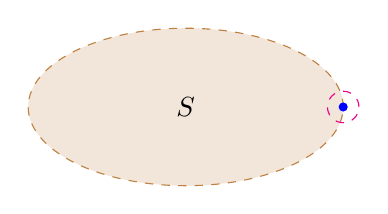
\begin{tikzpicture}
\draw[fill, brown!20!white, draw=brown, dashed] (5,0) ellipse [x radius=2cm, y radius=1cm];
\node[] () at (5,0) {\(S\)};
\draw[blue, fill] (7,0) circle [radius=0.5mm];
\draw[magenta, dashed] (7,0) circle [radius=2mm];
\end{tikzpicture}
\end{center}
\begin{remark}
\item Roughly speaking, an adherent point of \(S\) is a point that can be
``stuck'' to the set \(S\) (``touches'' or ``barely touches'' \(S\)).
\item Since every point \(x\in S\) must be an adherent point of \(S\) (\(B_X(x,r)\cap
S\) contains the point \(x\) at least, for any \(r>0\)), it follows that
\(S\subseteq \overline{S}\).
\item Since every adherent point of \(S\) must belong to \(X\), it follows that
\(\overline{S}\subseteq X\).
\end{remark}

\item The following result explains why \(\overline{S}\) is called ``closure''
of \(S\): Because it is the smallest \emph{closed} subset of \(X\) which
contains all points in \(S\).

\begin{theorem}
\label{thm:closure-smallest-closed}
The closure \(\overline{S}\) is the smallest closed subset of \(X\) which
contains all points in \(S\).\footnote{This means that for any closed subset
\(C\) of \(X\) which contains all points in \(S\), we have
\(\overline{S}\subseteq C\).}
\end{theorem}
\begin{pf}
Firstly, we will show that \(\overline{S}\) is closed in \(X\). Fix any \(x\in
X\setminus\overline{S}\) (i.e., any point in \(X\) that is not an adherent
point of \(S\)). Then, there exists \(r>0\) such that \(B_X(x,r)\cap
S=\varnothing\) by definition. This means that all points in \(B_X(x,r)\) do
not belong to \(S\), which implies that \(B_X(x,r)\subseteq X\setminus S\).

Now, take any \(y\in B_X(x,r)\). Then, by triangle inequality,
\[
B_X(y,r-d(x,y))=\{z\in X:d(y,z)<r-d(x,y)\}\subseteq \{z\in X:d(x,z)<r\}=B_X(x,r)\subseteq X\setminus S,
\]
which means that \(B_X(y,r-d(x,y))\cap S=\varnothing\), and thus \(y\in
X\setminus\overline{S}\). Since \(y\) is arbitrarily chosen from \(B_X(x,r)\),
we conclude that \(B_X(x,r)\subseteq X\setminus \overline{S}\), and so
\(X\setminus\overline{S}\) is open in \(X\), i.e., \(\overline{S}\) is closed
in \(X\).

Secondly, we will show that \(\overline{S}\) is the \emph{smallest} closed
subset of \(X\) which contains all points in \(S\). Let \(C\) be a closed
subset of \(X\) which contains all points in \(S\), i.e., \(C\supseteq S\). We
then have \(X\setminus C\subseteq X\setminus S\). Now, fix any \(x\in
X\setminus C\). Since \(X\setminus C\) is open, there exists \(r>0\) such that
\(x\in B_X(x,r)\subseteq X\setminus C\subseteq X\setminus S\). This implies
that \(B_X(x,r)\cap S=\varnothing\) for this \(r\), and so \(x\) is not an
adherent point of \(S\), i.e., \(x\in X\setminus\overline{S}\).

Since \(x\) is arbitrarily chosen from \(X\setminus C\), we conclude that
\(X\setminus C\subseteq X\setminus\overline{S}\), or \(\overline{S}\subseteq
C\).
\end{pf}

\item Another way to view the concept of adherent point is to consider the
notion of \emph{distance between a point and a set} (discussed in
\Cref{subsect:pt-set-dist}). We have the following criterion for
adherent point:
\begin{proposition}
\label{prp:adherent-zero-dist-from-set}
Let \(S\) be a subset of \(X\). A point \(x\in X\) is an adherent point of
\(S\) iff \(d(x,S)=0\).
\end{proposition}
\begin{pf}
Note that
\begin{align*}
&\hspace{1cm}\text{\(x\) is an adherent point of \(S\)}\\
&\iff \text{for any \(r>0\), \(B_X(x,r)\cap S\ne\varnothing\)}\\
&\iff\text{for any \(r>0\), there exists \(s_r\in S\) such that \(d(x,s_r)<r\)}\\
&\iff \inf_{s\in S}d(x,s)=0\\
&\iff d(x,S)=0.
\end{align*}
\end{pf}

\item Next, we will introduce the notion of \emph{accumulation point}. Let
\(S\) be a subset of \(X\). A point \(x\in X\) is an \defn{accumulation point}
of \(S\) (or \defn{limit point} of \(S\)) if it is an adherent point of
\(S\setminus\{x\}\), i.e., \(B(x,r)\cap(S\setminus\{x\})\ne\varnothing\) for
any \(r>0\). The set of all accumulation points of \(S\) (in \(X\)) is called
the \defn{derived set} of \(S\) in \(X\), and is denoted by \defn{\(S'\)}.


\begin{intuition}
A point is an accumulation point when there are \emph{other} points which are
``arbitrarily close'' to it (``accumulating'' to that point).
\begin{center}
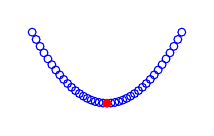
\begin{tikzpicture}
\foreach \x in {0.05,0.1,...,1} \draw[blue] (\x, \x^2) circle [radius=0.5mm];
\foreach \x in {0.05,0.1,...,1} \draw[blue] (-\x, \x^2) circle [radius=0.5mm];
\draw[red, fill] (0,0) circle [radius=0.5mm];
\end{tikzpicture}
\end{center}
\end{intuition}


\item The concepts of accumulation point and adherent point are similar, and
the only difference is ``\(\setminus\{x\}\)''. Since
\(B(x,r)\cap(S\setminus\{x\})\ne\varnothing\) implies \(B_X(x,r)\cap
S\ne\varnothing\), it follows that every accumulation point of \(S\) must also
be an adherent point of \(S\) (but not vice versa), i.e., \(S'\subseteq
\overline{S}\) (but the equality may not hold).

Example: Let \(S=(0,1)\cup\{2\}\). Then, \(S'=[0,1]\) while
\(\overline{S}=[0,1]\cup\{2\}\). \begin{note} \(2\) is not an accumulation
point of \(S\) since \(B(2,r)\cap (S{\color{red}\setminus\{2\}})\) is empty
when \(r=1/2\), but \(2\) is an adherent point of \(S\) as \(B(2,r)\cap
S\supseteq \{2\}\) for any \(r>0\).
\end{note} For this example, we can observe that \(2\) is ``isolated'' from
other points in \(S\). This motivates the definition of \emph{isolated point}.

\item Let \(S\) be a subset of \(X\). A point \(x\in S\) is an \defn{isolated
point} of \(S\) if there exists \(r>0\) such that \(B(x,r)\cap S=\{x\}\).
\begin{center}
\begin{tikzpicture}
\draw[-Latex] (0,0) -- (10,0);
\node[] () at (3,0) {(};
\node[] () at (5,0) {)};
\node[] () at (3,-0.5) {\(0\)};
\node[] () at (5,-0.5) {\(1\)};
\draw[line width=0.1cm, opacity=0.3, blue] (3,0) -- (5,0);
\node[blue] () at (7,-0.5) {\(2\)};
\draw[fill, blue] (7,0) circle [radius=0.5mm];
\node[green!50!black] () at (6.8,0) {(};
\node[green!50!black] () at (7.2,0) {)};
\draw[-Latex] (8,-0.6) -- (7,-0.1)
node[pos=-0.5]{``alone'' and ``isolated''};
\end{tikzpicture}
\end{center}


\item We can express the closure \(\overline{S}\) as a union of the derived set
\(S'\) and the set \(S\) itself:
\begin{proposition}
\label{prp:clos-union-deriv-s}
Let \(S\) be a subset of \(X\). Then, \(\overline{S}=S'\cup S\).
\end{proposition}
\begin{pf}
``\(\supseteq\)'': First, we have \(S'\subseteq \overline{S}\) and \(S\subseteq
\overline{S}\). Thus, \(S'\cup S\subseteq \overline{S}\).

``\(\subseteq\)'': For any \(x\in\overline{S}\), if \(x\in S\), we immediately
have \(x\in S'\cup S\). So henceforth we assume \(x\notin S\). Then, since
\(x\) is an adherent point of \(S\), we have for any \(r>0\),
\[
B(x,r)\cap S\ne\varnothing.
\]
Furthermore, since \(x\notin S\), we have \(S=S\setminus\{x\}\), so we indeed
have
\[
B(x,r)\cap (S\setminus\{x\})\ne\varnothing
\]
for any \(r>0\). This means that \(x\in S'\subseteq S'\cup S\).
\end{pf}

\item \label{it:isolated-point-equiv-def} Note that an isolated point \(x\in
S\) is the same as an adherent point of \(S\) which is \emph{not} an
accumulation point of \(S\).

\begin{pf}
``\(\Rightarrow\)'': Since \(x\in S\), \(x\) must be an adherent point of
\(S\). Also, there exists \(r>0\) such that \(B(x,r)\cap S=\{x\}\), so \(x\) is
not an accumulation point of \(S\).

``\(\Leftarrow\)'': When a point \(x\) is an adherent point of \(S\) but is not
an accumulation point of \(S\), we have:
\begin{itemize}
\item \(B(x,r)\cap S\ne\varnothing\) for any \(r>0\), and
\item \(B(x,r_0)\cap (S\setminus\{x\})=\varnothing\) for some \(r_0>0\).
\end{itemize}
This then forces that \(B(x,r_0)\cap S=\{x\}\) for the \(r_0\), so \(x\) is an
isolated point of \(S\).
\end{pf}

\item\label{it:closure-decompose-acc-isolate} Therefore, we can indeed express
the closure \(\overline{S}\) as a \emph{disjoint union} of the derived set
\(S'\) and the \emph{set of all isolated points of \(S\)}, denoted by \(S^i\):
\[
\overline{S}=S'\sqcup S^{i}.
\]

\item It turns out that we can give an criterion for being an
accumulation point by considering \emph{cardinality}.
\begin{proposition}
\label{prp:acc-pt-inf-set}
Let \(S\) be a subset of \(X\) and \(x\in X\). Then, \(x\) is an accumulation
point of \(S\) iff \(B(x,r)\cap S\) is an infinite set for any \(r>0\).
\end{proposition}
\begin{pf}
``\(\Rightarrow\)'': Assume to the contrary that \(x\) is an accumulation point
of \(S\) while \(B(x,r)\cap S\) is a finite set for some \(r>0\). Since
\(B(x,r)\cap S\) is a finite set, we can pick a \(y\in B(x,r)\cap S\) which has
the \emph{minimum} distance from \(x\) (call it \(r_0\)).

Then, consider the open ball \(B(x,r_0/2)\). By construction of \(r_0\),
\(B(x,r_0/2)\cap (S\setminus\{x\})\) must be empty. This contradicts to the
assumption that \(x\) is an accumulation point of \(S\).

``\(\Leftarrow\)'': Straightforward since when \(B(x,r)\cap S\) is an
\emph{infinite} set for any \(r>0\), it must still contain elements after
taking away \(x\) (for any \(r>0\)), i.e., \(B(x,r)\cap
(S\setminus\{x\})\ne\varnothing\) for any \(r>0\).
\end{pf}

\item Next, we will introduce a result that gives criteria for
\emph{closedness} of a set, using the notion of closure and derived set.

\begin{proposition}
\label{prp:equiv-crit-closed}
Let \(S\) be a subset of \(X\). Then, the following are equivalent.
\begin{enumerate}
\item \(S\) is closed in \(X\).
\item \(S'\subseteq S\).
\item \(\overline{S}=S\).
\end{enumerate}
\end{proposition}
\begin{pf}
\underline{\(\text{(a)}\implies \text{(b)}\)}: Assume to the contrary that
\(S\) is closed in \(X\) and \(S'\) is \emph{not} a subset of \(S\). Then,
there exists \(x\in S'\setminus S\subseteq X\setminus S\). But since \(S\) is
closed in \(X\), i.e., \(X\setminus S\) is open in \(X\), there must exist
\(r>0\) such that \(B(x,r)\subseteq X\setminus S\), which means \(B(x,r)\cap
S=\varnothing\). This then contradicts to \(x\in S'\) (\(x\) is an accumulation
point, hence adherent point of \(S\)).

\underline{\(\text{(b)}\implies \text{(c)}\)}: Assume that \(S'\subseteq S\).
Then, by \Cref{prp:clos-union-deriv-s}, we have \(\overline{S}=S'\cup S=S\).

\underline{\(\text{(c)}\implies \text{(a)}\)}: Assume that \(\overline{S}=S\).
By \Cref{thm:closure-smallest-closed}, we know that \(\overline{S}\) is closed
in \(X\), so does \(S\).
\end{pf}

\item Then, we will introduce the notion of \emph{boundary point}.
\begin{center}
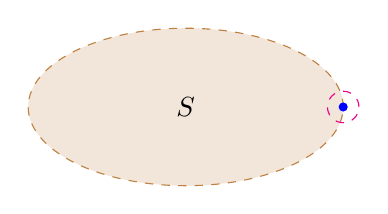
\begin{tikzpicture}
\draw[fill, brown!20!white, draw=brown, dashed] (5,0) ellipse [x radius=2cm, y radius=1cm];
\node[] () at (5,0) {\(S\)};
\draw[blue, fill] (7,0) circle [radius=0.5mm];
\draw[magenta, dashed] (7,0) circle [radius=2mm];
\end{tikzpicture}
\end{center}
We would like to capture the intuitive notion of ``a point located at the
`boundary' of \(S\)'' by \emph{boundary point}. From the picture above, we
observe that for a point that lies on the ``boundary'', every open ball
centered at that point contains some elements in \(S\) as well as some elements
\emph{not} in \(S\), no matter how small the ball is. This leads to the
following definition of boundary point.

\item Let \(S\subseteq X\) be a subset. A point \(x\in X\) is a \defn{boundary
point} of \(S\) if \(B(x,r)\cap S\ne\varnothing\) and \(B(x,r)\cap (X\setminus
S)\ne\varnothing\) for any \(r>0\). The set of all boundary points of \(S\) is
called the \defn{boundary} of \(S\), and is denoted by \defn{\(\partial S\)}.

\begin{remark}
\item By definition, we can write \(\partial
S=\overline{S}\cap\overline{X\setminus S}\subseteq\overline{S}\). This
implies that \(\partial S=\partial(X\setminus S)\) and \(\partial S\) is closed
in \(X\) (as an intersection of two closed subsets in \(X\)).
\item Note that \(S^{\circ}\cap \partial S=\varnothing\). This is because for
any interior point \(x\) of \(S\), we need \(B(x,r)\subseteq S\) for any
\(r>0\), so the ball \(B(x,r)\) cannot possibly contain elements outside \(S\),
failing a requirement for being a boundary point of \(S\). This shows that a
point cannot possibly be simultaneously interior point and boundary point of
\(S\).
\end{remark}

The notion of boundary here coincides with our usual understanding of
``boundary''. For example, when \(X=\R^n\), the boundary of an open ball
\(B(a,r)\) (``solid'' \(n\)-ball) is
\[
\partial B(x,r)=\{y\in\R^n:d(x,y)=r\},
\]
an \emph{\(n\)-sphere} (which is the ``boundary''/``surface'' of the ball in
our usual understanding).

\item \label{it:closure-decompose-bound-interior} Recall from
\labelcref{it:closure-decompose-acc-isolate} that we can express the closure
\(\overline{S}\) as the disjoint union of a set containing all accumulation
points and another set containing all isolated points.

Using the concept of \emph{boundary points} and \emph{interior points}, we can
express the closure \(\overline{S}\) in a similar fashion as follows:
\[
\overline{S}=\partial S\sqcup S^{\circ}.
\]
\begin{pf}
From the remarks above, we know that \(S^{\circ}\cap \partial S=\varnothing\).
So it suffices to show that \(\overline{S}=\partial S\cup S^{\circ}\).

``\(\supseteq\)'': We have \(\partial S\subseteq S\) as noted in the previous
remarks, and also we have \(S^{\circ}\subseteq S\subseteq \overline{S}\). Thus,
the union \(\partial S\cup S^{\circ}\subseteq S\).

``\(\subseteq\)'': Fix any \(x\in\overline{S}\). If \(x\in S^{\circ}\), then we
are done. So henceforth assume that \(x\notin S^{\circ}\). In this case, we
must have \(B(x,r)\cap (X\setminus S)\ne\varnothing\) (i.e., \(B(x,r)\) is not
a subset of \(S\)) for any \(r>0\). Also, since \(x\in\overline{S}\), we have
\(B(x,r)\cap S\ne\varnothing\) for any \(r>0\). It follows that \(x\in\partial
S\subseteq \partial S\cup S^{\circ}\).
\end{pf}
\end{enumerate}
\subsection{Properties of Interiors, Closures, Derived Sets, and Boundaries}
\label{subsect:int-clos-deriv-bound-prop}
\begin{enumerate}
\item So far we have introduced multiple kinds of \emph{points}, including:
\begin{enumerate}
\item interior points \faIcon{arrows-alt-h} interior \(S^{\circ}\)
\item adherent points \faIcon{arrows-alt-h} closure \(\overline{S}\)
\item accumulation points \faIcon{arrows-alt-h} derived set \(S'\)
\item boundary points \faIcon{arrows-alt-h} boundary \(\partial S\)
\end{enumerate}
In \Cref{subsect:int-clos-deriv-bound-prop} we will discuss some set-related
properties about them. Throughout we let \((X,d)\) be a metric space and
\(S,T\) be arbitrary subsets of \(X\).

\item \label{it:interior-set-prop}
Properties for interior \(S^{\circ}\):
\begin{enumerate}
\item\label{it:int-pre-subset} (preserving subset inclusion) \(S\subseteq
T\implies S^{\circ}\subseteq T^{\circ}\).

\begin{pf}
Assume \(S\subseteq T\). For any \(s\in S^{\circ}\), there exists \(r>0\) such
that \(B(s,r)\subseteq S\subseteq T\), so \(s\in T^{\circ}\). Hence
\(S^{\circ}\subseteq T^{\circ}\).
\end{pf}
\item \label{it:int-idempot} (idempotence) \((S^{\circ})^{\circ}=S^{\circ}\).

\begin{pf}
We need to show that \(S^{\circ}\) is open in \(X\). Fix any \(x\in
S^{\circ}\). Then there exists \(r>0\) such that \(B(x,r)\subseteq S\).

It then suffices to show that \(B(x,r)\subseteq S^{\circ}\). First fix any
\(y\in B(x,r)\). By the openness of \(B(x,r)\), there exists \(\delta>0\) such
that \(B(y,\delta)\subseteq B(x,r)\subseteq S\), which implies that \(y\) is
also an interior point of \(S\), i.e., \(y\in S^{\circ}\). This shows
\(B(x,r)\subseteq S^{\circ}\).
\end{pf}
\item \(S^{\circ}\subseteq T\subseteq S\implies T^{\circ}=S^{\circ}\).

\begin{pf}
By \labelcref{it:int-pre-subset,it:int-idempot},
\[
S^{\circ}\subseteq T\subseteq S\implies 
S^{\circ}=(S^{\circ})^{\circ}\subseteq T^{\circ}\subseteq S^{\circ}
\implies T^{\circ}=S^{\circ}.
\]
\end{pf}
\item (commutativity with intersection) \(S^{\circ}\cap T^{\circ}=(S\cap
T)^{\circ}\).

\begin{pf}
``\(\subseteq\)'': Fix any \(x\in S^{\circ}\cap T^{\circ}\). Then there exist
\(r_1,r_2>0\) such that \(B(x,r_1)\subseteq S\) and \(B(x,r_2)\subseteq T\).
Let \(r=\min\{r_1,r_2\}>0\), and we have \(B(x,r)\subseteq S\cap T\). Thus,
\(x\in(S\cap T)^{\circ}\).

``\(\supseteq\)'': Note that \(S\cap T\subseteq S\) and \(S\cap T\subseteq T\).
Thus, by \labelcref{it:int-pre-subset}, we have
\[
(S\cap T)^{\circ}\subseteq S^{\circ}\qqtext{and}
(S\cap T)^{\circ}\subseteq T^{\circ}.
\]
This means \((S\cap T)^{\circ}\subseteq S^{\circ}\cap T^{\circ}\).
\end{pf}
\item \(S^{\circ}\cup T^{\circ}\subseteq (S\cup T)^{\circ}\).

\begin{pf}
We have \(S\subseteq S\cup T\) and \(T\subseteq S\cup T\).
Thus, by \labelcref{it:int-pre-subset}, \(S^{\circ}\subseteq
(S\cup T)^{\circ}\) and \(T^{\circ}\subseteq (S\cup T)^{\circ}\). Hence,
\[
S^{\circ}\cup T^{\circ}\subseteq (S\cup T)^{\circ}.
\]
\end{pf}

\begin{warning}
It is \underline{not} true that \(S^{\circ}\cup T^{\circ}\supseteq (S\cup
T)^{\circ}\). For example, consider \(S=[0,1]\) and \(T=[1,2]\) in \(\R\).
\end{warning}
\end{enumerate}

\item \label{it:clos-set-prop}
Properties for closure \(\overline{S}\):
\begin{enumerate}
\item \label{it:clos-pre-subset} (preserving subset inclusion) \(S\subseteq
T\implies \overline{S}\subseteq \overline{T}\).

\begin{pf}
Assume \(S\subseteq T\).  For any \(x\in\overline{S}\) and any \(r>0\), we have
\[
B(x,r)\cap T\supseteq B(x,r)\cap S\ne\varnothing,
\]
which implies \(B(x,r)\cap T\ne\varnothing\), so \(x\in \overline{T}\).
\end{pf}
\item \label{it:clos-idempot} (idempotence) \(\overline{(\overline{S})}=\overline{S}\).

\begin{pf}
Note that \(\overline{S}\) is closed, and hence the smallest closed set in
\(X\) containing all elements in \(\overline{S}\) is precisely \(\overline{S}\)
itself. This means that \(\overline{(\overline{S})}=\overline{S}\) by
\Cref{thm:closure-smallest-closed}.
\end{pf}
\item \(S\subseteq T\subseteq \overline{S}\implies \overline{T}=\overline{S}\).

\begin{pf}
By \labelcref{it:clos-pre-subset,it:clos-idempot}, we have
\[
S\subseteq T\subseteq \overline{S}
\implies
\overline{S}\subseteq \overline{T}\subseteq \overline{(\overline{S})}=\overline{S}
\implies
\overline{T}=\overline{S}.
\]
\end{pf}
\item (commutativity with union) \(\overline{S}\cup\overline{T}=\overline{S\cup T}\).

\begin{pf}
``\(\subseteq\)'':  We have \(S\subseteq S\cup T\) and \(T\subseteq S\cup T\).
Thus, by \labelcref{it:clos-pre-subset}, \(\overline{S}\subseteq
\overline{S\cup T}\) and \(\overline{T}\subseteq \overline{S\cup T}\). Hence,
\[
\overline{S}\cup\overline{T}\subseteq \overline{S\cup T}.
\]
``\(\supseteq\)'': Fix any \(x\in\overline{S\cup T}\) and any \(r>0\). Then we
have
\begin{equation}
\label{eq:clos-union-rev-subs}
[B(x,r)\cap S]\cup[B(x,r)\cap T]=B(x,r)\cap(S\cup T)\ne\varnothing.
\end{equation}
If \(B(x,r)\cap S\ne\varnothing\) for any \(r>0\), then
\(x\in\overline{S}\subseteq \overline{S}\cup\overline{T}\) and we are done.
So henceforth assume that \(B(x,r_0)\cap S=\varnothing\) for some \(r_0>0\). Then,
\[
B(x,r)\cap S=\varnothing
\]
for any \(0<r\le r_0\). By \Cref{eq:clos-union-rev-subs}, we must have
\(B(x,r)\cap T\ne\varnothing\) for any \(0<r\le r_0\). Also, for any \(r>r_0\)
we have
\[
B(x,r)\cap T\supseteq B(x,r_0)\cap T\ne\varnothing.
\]
Hence, we conclude that \(B(x,r)\cap T\ne\varnothing\) for any \(r>0\), thus
\(x\in\overline{T}\subseteq \overline{S}\cup\overline{T}\).
\end{pf}
\item \(\overline{S}\cap\overline{T}\supseteq\overline{S\cap T}\).

\begin{pf}
Note that \(S\cap T\subseteq S\) and \(S\cap T\subseteq T\). Hence, by
\labelcref{it:clos-pre-subset}, we have \(\overline{S\cap T}\subseteq
\overline{S}\) and \(\overline{S\cap T}\subseteq \overline{T}\). Thus,
\[
\overline{S\cap T}\subseteq \overline{S}\cap\overline{T}.
\]
\end{pf}

\begin{warning}
It is \underline{not} true that
\(\overline{S}\cap\overline{T}\subseteq\overline{S\cap T}\). For example,
consider \(S=[0,1)\) and \(T=(1,2]\) in \(\R\).
\end{warning}

\end{enumerate}
\item \label{it:deriv-set-prop}
Properties for derived set \(S'\):
\begin{enumerate}
\item \label{it:deriv-pre-subset} (preserving subset inclusion) \(S\subseteq
T\implies S'\subseteq T'\).

\begin{pf}
Assume \(S\subseteq T\).  For any \(x\in S'\) and any \(r>0\), we have
\[
B(x,r)\cap T\setminus \{x\}\supseteq B(x,r)\cap S\setminus \{x\}\ne\varnothing,
\]
which implies \(B(x,r)\cap T\setminus \{x\}\ne\varnothing\), so \(x\in T'\).
\end{pf}
\item \((S')'\subseteq S'\).

\begin{pf}
Fix any \(x\in(S')'\) and any \(r>0\). Then there exists \(y\in B(x,r)\cap
S'\setminus \{x\}\). Let \(\delta=r-d(x,y)>0\). Then,
\[
B(y,\delta)\subseteq B(x,r).
\]
Since \(y\in S'\), by \Cref{prp:acc-pt-inf-set} we know that \(B(y,\delta)\cap
S\setminus \{y\}\) is infinite, so we can find an element other than \(x\) in
it. In other words, there exists
\[
z\in B(y,\delta)\cap S\setminus \{x,y\}
\subseteq B(x,r)\cap S\setminus \{x\},
\]
which implies that \(B(x,r)\cap S\setminus \{x\}\) is nonempty, so \(x\in S'\).
\end{pf}

\begin{warning}
It is \underline{not} true that \((S')'\supseteq S'\). For example, consider
\(S=\{1/n:n\in\N\}\) in \(\R\).
\end{warning}
\item (commutativity with union) \(S'\cup T'=(S\cup T)'\).

\begin{pf}
Similar to the proof for the respective property for closure.
\end{pf}
\item \(S'\cap T'\supseteq (S\cap T)'\).

\begin{pf}
Similar to the proof for the respective property for closure.
\end{pf}

\begin{warning}
It is \underline{not} true that \(S'\cap T'\subseteq (S\cap T)'\). For example, consider
\(S=[0,1)\) and \(T=(1,2]\) in \(\R\).
\end{warning}
\end{enumerate}

\item \label{it:bound-prop}
Properties for boundary \(\partial S\):
\begin{enumerate}
\item \(\partial(\partial S)\subseteq \partial S\).

\begin{pf}
Firstly, since \(\partial S=\overline{S}\cap\overline{X\setminus S}\) and
closure is closed, we know that \(\partial S\) is closed in \(X\), which
implies that \(\overline{\partial S}=\partial S\). Thus,
\[
\partial(\partial S)=\overline{\partial S}\cap\overline{X\setminus \partial S}
\subseteq \overline{\partial S}=\partial S
\]
\end{pf}

\begin{warning}
It is \underline{not} true that \(\partial(\partial S)\supseteq \partial S\). For example, consider
\(S=\Q\) in \(\R\).
\end{warning}
\item \(\partial(S\cup T)\subseteq \partial S\cup\partial T\).

\begin{pf}
Note that
\begin{align*}
\partial(S\cup T)
&=\overline{S\cup T}\cap\overline{X\setminus (S\cup T)}\\
&=\overline{S\cup T}\cap\overline{(X\setminus S)\cap (X\setminus T)}\\
&=(\overline{S}\cup\overline{T})\cap\overline{(X\setminus S)\cap (X\setminus T)}\\
&\subseteq (\overline{S}\cup\overline{T})\cap\vc{(\overline{X\setminus S}\cap\overline{X\setminus T})}\\
&= [\overline{S}\cap\vc{(\overline{X\setminus S}\cap\overline{X\setminus T})}]\cup
[\overline{T}\cap\vc{(\overline{X\setminus S}\cap\overline{X\setminus T})}]\\
&\subseteq [\overline{S}\cap\overline{X\setminus S}]\cup
[\overline{T}\cap\overline{X\setminus T}]\\
&=\partial S\cup\partial T.
\end{align*}
\end{pf}

\begin{warning}
It is \underline{not} true that \(\partial(S\cup T)\supseteq \partial
S\cup\partial T\). For example, consider \(S=[0,2]\) and \(T=\{1\}\) in \(\R\).
\end{warning}
\item \label{it:bound-inter-subset} \(\partial(S\cap T)\subseteq \partial S\cup\partial T\).

\begin{pf}
Note that
\begin{align*}
\partial(S\cap T)
&=\overline{S\cap T}\cap\overline{X\setminus (S\cap T)}\\
&=\overline{S\cap T}\cap\overline{(X\setminus S)\cup (X\setminus T)}\\
&=\overline{S\cap T}\cap (\overline{X\setminus S}\cup \overline{X\setminus T})\\
&\subseteq \vc{(\overline{S}\cap\overline{T})}\cap(\overline{X\setminus S}\cup \overline{X\setminus T})\\
&=[\vc{(\overline{S}\cap\overline{T})}\cap\overline{X\setminus S}]
\cup[\vc{(\overline{S}\cap\overline{T})}\cap\overline{X\setminus T}]\\
&\subseteq (\overline{S}\cap\overline{X\setminus S})
\cup(\overline{T}\cap\overline{X\setminus T})\\
&=\partial S\cup\partial T.
\end{align*}
\end{pf}

\begin{warning}
It is \underline{not} true that \(\partial(S\cap T)\supseteq \partial
S\cup\partial T\). For example, consider \(S=[0,1]\) and \(T=\{2\}\) in \(\R\).
\end{warning}

\item \(\partial(S\setminus T)\subseteq \partial S\cup\partial T\).

\begin{pf}
Note that \(\partial S=\partial(X\setminus S)\). Thus, by
\labelcref{it:bound-inter-subset} we have
\[
\partial(S\setminus T)=\partial(S\cap(X\setminus T))
\subseteq \partial S\cup\partial(X\setminus T)
=\partial S\cup\partial T.
\]
\end{pf}

\begin{warning}
It is \underline{not} true that \(\partial(S\setminus T)\supseteq \partial
S\cup\partial T\). For example, consider \(S=[0,1]\) and \(T=\{2\}\) in \(\R\).
\end{warning}
\end{enumerate}
\end{enumerate}
\subsection{Compactness}
\label{subsect:compactness}
\begin{enumerate}
\item We have introduced the concept of \emph{open set} and \emph{closed set}.
They can be seen as generalizations to the concept of \emph{open interval} and
\emph{closed interval} in \(\R\) respectively. However, when we consider a more
general notion like open or closed set instead of a more ``specialized'' notion
like open or closed interval, some properties may be lost.

\item For example, consider the case in \(\R\). For a \emph{closed interval}
\([a,b]\) (\(a,b\in\R\)), we have the \emph{extreme value theorem} which states
that for any function \(f\in C[a,b]\) (\(C[a,b]\) denotes the set of all
continuous functions from \([a,b]\) to \(\R\)), \(f\) attains its maximum and
minimum. More specifically, there exist \(c,d\in[a,b]\) such that
\[
f(c)=\min\{f(x):x\in [a,b]\}
\]
and
\[
f(d)=\max\{f(x):x\in[a,b]\}.
\]
This property may \emph{not} hold for closed set (even in \(\R\)) \warn{}. For
example, \([0,\infty)\) is a closed set in \(\R\) (but \emph{not} a closed
interval). A continuous function defined on \([0,\infty)\) can be
\emph{unbounded} (so such maximum and minimum \emph{do not even exist}!).

\item To preserve this property from extreme value theorem, we thus need to
enforce additional constraint on closed sets. It turns out that by restricting
our attention to \emph{compact sets}, the property is preserved.  We shall
discuss the notion of \emph{compactness} in \Cref{subsect:compactness}.

\item Before defining compactness, we need to introduce some preliminary
terminologies. Let \((X,d)\) be a metric space throughout
\Cref{subsect:compactness}. Let \(S\) be a subset of \(X\). Then, a family
\(\mathcal{F}\) of subsets of \(X\) is said to be a \defn{cover} of \(S\) (in
\(X\)) if
\[
\bigcup_{F\in\mathcal{F}}F\supseteq S,
\]
i.e., the union of all the family members in \(\mathcal{F}\) contains all
elements in \(S\). If every \(F\in\mathcal{F}\) is open in \(X\), then
\(\mathcal{F}\) is called an \defn{open cover} of \(S\).

\begin{intuition}
All the sets in a cover \(\mathcal{F}\) of \(S\) altogether provide a complete
``coverage'' of \(S\), hence the name ``cover''.
\end{intuition}
\item The following pictures illustrate graphically what \emph{covers} look like:
\begin{center}
\begin{tikzpicture}
\draw[-Latex] (0,0) -- (10,0);
\node[blue] () at (3,0) {(};
\node[blue] () at (7,0) {)};
\draw[blue, very thick] (3,0) -- (7,0)
node[midway, above]{\(S=(0,1)\)};
\node[] () at (3,-0.7) {\(0\)};
\node[] () at (7,-0.7) {\(1\)};
\foreach \x in {2.6, 2.9, ..., 7.4} {
\node[orange, opacity=0.7] () at (\x,0) {(};
\node[orange, opacity=0.7] () at (\x+0.3,0) {)};
\draw[line width=0.1cm, opacity=0.6, yellow, line cap=round] (\x,0) -- (\x+0.3,0);
\draw[-Latex] (5,-1) -- (\x+0.15,-0.2);
}
\node[] () at (5,-1.5) {forming an open cover of \(S\)};
\end{tikzpicture}
\begin{tikzpicture}
\draw[-Latex] (-3,0) -- (3,0);
\draw[-Latex] (0,-3) -- (0,3);
\node[draw] () at (4.5,1) {\(S=\R^2\)};
\foreach \x in {-2.8,-2.4,...,2.8}
\foreach \y in {-2.8,-2.4,...,2.8}
{
\draw[dashed, orange, opacity=0.4, fill=yellow] (\x,\y) circle [radius=10pt];
}
\node[] () at (0,-3.5) {forming an open cover of \(S\)};
\end{tikzpicture}
\begin{tikzpicture}
\draw[-Latex] (-3,0) -- (3,0);
\draw[-Latex] (0,-3) -- (0,3);
\node[draw] () at (4.5,1) {\(S=\R^2\)};
\foreach \x in {-2.8,-2.1,...,2.8}
\foreach \y in {-2.8,-2.1,...,2.8}
{
\draw[dashed, orange, opacity=0.4, fill=yellow] (\x,\y) circle [radius=10pt];
}
\node[] () at (0,-3.5) {\emph{not} forming an open cover of \(S\) (there are some ``gaps'')};
\end{tikzpicture}
\end{center}
\item The following gives some concrete examples of covers. Let \(X=\R\) here
(and \(d\) be the standard Euclidean distance).
\begin{enumerate}
\item\label{it:example-01-cover} \(\mathcal{F}=\{(x-1/2,x+1/2):x\in[0,1]\}\) is an open cover of
\([0,1]\).
\begin{center}
\begin{tikzpicture}
\draw[-Latex] (0,0) -- (10,0);
\node[blue] () at (3,0) {[};
\node[blue] () at (7,0) {]};
\draw[blue, very thick] (3,0) -- (7,0)
node[midway, above]{\(S=[0,1]\)};
\node[] () at (3,-0.7) {\(0\)};
\node[] () at (7,-0.7) {\(1\)};
\foreach \x in {3, 3.02, ..., 7} {
\node[orange, opacity=0.7] () at (\x-2,0) {(};
\node[orange, opacity=0.7] () at (\x+2,0) {)};
\draw[line width=0.1cm, opacity=0.6, yellow, line cap=round] (\x-2,0) -- (\x+2,0);
}
\end{tikzpicture}
\end{center}
It is an \emph{uncountable} cover of \([0,1]\). From the picture we can observe
that there are indeed many \emph{redundancies} in the family. We do not really
need uncountably many members to cover \([0,1]\)! In fact, having only
\emph{two} of them is sufficient to cover \([0,1]\): We can pick
\((1/4-1/2,1/4+1/2)=(-1/4,3/4)\) and \((3/4-1/2,3/4+1/2)=(1/4,5/4)\). Then,
we have \[(-1/4,3/4)\cup (1/4,5/4)=(-1/4,5/4)\supseteq [0,1].\] Thus, the
\emph{finite} set \(\mathcal{F}_0=\{(-1/4,3/4),(1/4,5/4)\}\) can already serve
as an open cover of \([0,1]\).
\begin{note}
Since \(\mathcal{F}_0\) is formed by members picked from the original cover
\(\mathcal{F}\), sometimes we call \(\mathcal{F}_0\) as a \emph{subcover} of
\(\mathcal{F}\).

More generally, given any cover \(\mathcal{F}\) of a set \(S\), a family
\(\mathcal{G}\) is said to be a \defn{subcover} of \(\mathcal{F}\) if
\(\mathcal{G}\subseteq \mathcal{F}\) and \(\mathcal{G}\) is also a cover of
\(S\).
\end{note}
\item \label{it:example-r-cover-int} \(\mathcal{F}=\{(n-1,n+1):n\in\Z\}\) is an open cover of \(\R\).
\begin{center}
\begin{tikzpicture}
\draw[-Latex] (-5,0) -- (5,0);
\node[draw] () at (0,1) {\(S=\R\)};
\foreach \x in {-4, -3, ..., 4} {
\node[] () at (\x, -0.5) {\(\x\)};
\node[orange, opacity=0.7] () at (\x-1,0) {(};
\node[orange, opacity=0.7] () at (\x+1,0) {)};
\draw[line width=0.1cm, opacity=0.6, yellow, line cap=round] (\x-1,0) -- (\x+1,0);
}
\end{tikzpicture}
\end{center}
\end{enumerate}
\item Now, we are ready to introduce the notion of \emph{compactness}. A set
\(S\subseteq X\) is said to be \defn{compact} if every open cover of \(S\) has
a finite subcover.

Examples:
\begin{itemize}
\item The open cover \(\mathcal{F}\) in \labelcref{it:example-01-cover} has
a finite subcover, namely \(\mathcal{F}_0=\{(-1/4,3/4),(1/4,5/4)\}\).
\item The open cover \(\mathcal{F}\) in \labelcref{it:example-r-cover-int} does
\emph{not} have a finite subcover.

\begin{pf}
Assume to the contrary that it has a finite subcover
\(\mathcal{F}_0=\{(n-1,n+1):n\in S\}\) where \(S\) is a finite set of integers.
Let \(M\) be the maximum integer in the finite set \(S\). Then, note that the
real number \(M+1\) is not contained in any of the open intervals in
\(\mathcal{F}_0\), so \(\mathcal{F}_0\) is not a cover of \(\R\),
contradiction.
\end{pf}

This shows that \(\R\) is not compact (when \(X=\R\) and the metric is the
standard Euclidean distance).
\end{itemize}

\item The definition of a compact set may appear to be a bit technical and does
not convey too much information on the ``nature'' of the set. So in the
following we are going to prove some results that tell us more about what a
compact set ``looks like''. The first result suggests the \emph{closedness} and
\emph{boundedness} of a compact set.

\begin{theorem}
\label{thm:compact-imp-closed-bounded}
Every compact subset of \(X\) is closed (in \(X\)) and bounded.
\end{theorem}
\begin{pf}
Let \(S\subseteq X\) be any compact set. If \(S\) is empty, then its diameter
is conventionally set as \(-\infty\), which is not \(\infty\). Thus, it is
bounded. Also, we know from \Cref{prp:both-open-and-closed} that empty set must
be closed in \(X\). So we are done with this case.

Henceforth, we assume that \(S\ne\varnothing\). Fix any \(x\in S\). We first
show the \underline{boundedness}. Consider the open cover
\[
\mathcal{F}=\{B(x,n):n\in\N\}
\]
of \(S\). \begin{note}
We have \(B(x,1)\subseteq B(x,2)\subseteq B(x,3)\subseteq \dotsb\).
\end{note}
By the compactness, \(\mathcal{F}\) has a finite subcover \(\mathcal{F}_0\).
Then, we have
\[
\bigcup_{F\in\mathcal{F}_0}F\supseteq S.
\]
By the finiteness, we know that the union \(\displaystyle
\bigcup_{F\in\mathcal{F}_0}F\) must be a subset of a large open ball
\(B(x,M)\) where \(M\in\N\). Hence, for this \(M\), we have \(d(P,Q)\le
M\) for any \(P,Q\in S\), establishing the boundedness.

Next, we show the \underline{closedness}. By definition, it suffices to show
that \(X\setminus S\) is open in \(X\). Fix any \(p\in X\setminus S\). We would
like to find a \(r>0\) such that \(B(p,r)\subseteq X\setminus S\), i.e.,
\(B(p,r)\cap S=\varnothing\).

Since \(S\) is compact, the open cover \(\displaystyle
\mathcal{F}=\qty{B\qty(x,\frac{1}{2}d(x,p)):x\in S}\) of \(S\) has a finite subcover,
written as \(\{B(x_i,r_i):i=1,\dotsc,n\}\). Then we have
\[
\bigcup_{i=1}^{n}B(x_i,r_i)\supseteq S.
\]

Let \(r=\min\{r_1,\dotsc,r_n\}\).  Then, we can observe that \(B(p,r)\cap
B(x_i,r_i)=\varnothing\) for any \(i=1,\dotsc,n\), by the construction of the
open cover \(\mathcal{F}\).
\begin{center}
\begin{tikzpicture}
\draw[dashed] (-1,1) circle [radius=2cm];
\draw[blue, fill] (-1,1) circle [radius=0.05cm];
\node[blue] () at (-1,0.5) {\(x_1\)};
\draw[dashed] (3,1) circle [radius=2.5cm];
\draw[blue, fill] (3,1) circle [radius=0.05cm];
\node[blue] () at (3,0.5) {\(x_2\)};
\draw[blue, fill] (0.1,-2.9) circle [radius=0.05cm];
\node[blue] () at (0.1,-3.2) {\(p\)};
\draw[dashed, ForestGreen] (0.1,-2.9) circle [radius=2cm];
\draw[pen colour=orange, very thick, decorate,decoration={calligraphic brace, amplitude=5pt, raise=0}] (-0.4,-0.95) -- (0.1,-2.9)
node[midway, right=0.3cm, orange]{\(r=\min\{r_1,r_2\}\)};
\draw[pen colour=magenta, very thick, decorate,decoration={calligraphic brace, amplitude=5pt, raise=0}] (-1,1) -- (-0.4,-0.85)
node[midway, right=0.3cm, magenta]{\(r_1=d(x_1,p)/2\)};
\draw[pen colour=magenta, very thick, decorate,decoration={calligraphic brace, amplitude=5pt, raise=0}] (3,1) -- (1.3,-0.85)
node[midway, right=0.3cm, magenta]{\(r_2=d(x_2,p)/2\)};
\end{tikzpicture}
\end{center}
Since \(\displaystyle \bigcup_{i=1}^{n}B(x_i,r_i)\supseteq S\), it follows that
\(B(p,r)\cap S=\varnothing\) also. Thus, we conclude that \(S\) is closed in \(X\).
\end{pf}
\item The next one is about the so-called \emph{Boltzano-Weierstrass property}.
\begin{theorem}
\label{thm:cpt-bw-prop}
Every compact subset \(S\) of \(X\) has the \defn{Boltzano-Weierstrass
property}, i.e., every infinite subset of \(S\) has an accumulation point in \(S\).
\end{theorem}
\begin{pf}
Assume to the contrary that \(T\subseteq S\) is an infinite set with no
accumulation point in \(S\). Fix any \(s\in S\). Since \(s\) is \emph{not} an
accumulation point of \(T\), there exists an open ball \(B(s,r_s)\) containing
\(s\) such that \(B(s,r_s)\cap T=\varnothing\) (when \(s\notin T\)) or
\(B(s,r_s)\cap T=\{s\}\) (when \(s\in T\))

Now, as \(S\) is compact, the open cover \(\{B(s,r_s):s\in S\}\) of \(S\) has a
finite subcover \(\mathcal{F}_0\). Note that we then have
\[
\bigcup_{F\in\mathcal{F}_0}F\supseteq S\supseteq T.
\]
Since the union \(\displaystyle \bigcup_{F\in\mathcal{F}_0}F\) is finite (as
each family member contains either zero or one element), it implies that \(T\)
is finite also, contradiction.
\end{pf}
\item The following result describes the behaviour of \emph{closed subsets} of
a compact set.
\begin{theorem}
\label{thm:subset-closed-in-cpt-is-cpt}
Every closed subset of a compact set \(S\) (closed in \(S\)) is compact.
\end{theorem}
\begin{pf}
Let \(S\subseteq X\) be a compact set and \(T\subseteq S\) be a closed set in
\(S\). Let \(\mathcal{F}=\{U_{\lambda}:\lambda\in\Lambda\}\) be any open cover
of \(T\) \emph{in \(S\)}.

As \(T\) is closed in \(S\), by definition \(S\setminus T\) is open in \(S\).
Hence, \(\mathcal{F}\cup(S\setminus T)\) is an open cover of \(S\) in \(S\),
thus it has a finite sub-cover \(\mathcal{F}_0\). By adding the set
\(S\setminus T\) into \(\mathcal{F}_0\) if needed, we can assume that
\(S\setminus T\in\mathcal{F}_0\), so \(\mathcal{F}_0\) takes the form
\[
\{U_1,\dotsc,U_n,S\setminus T\}
\]
(with possibly relabelling for the indices). Hence, we have
\[
T\subseteq S\subseteq \qty(\bigcup_{i=1}^{n}U_i)\cup (S\setminus T).
\]
Since \(T\cap (S\setminus T)=\varnothing\), it follows that
\[
T\subseteq \bigcup_{i=1}^{n}U_i.
\]
Thus, the family \(\{U_1,\dotsc,U_n\}\) serves as a finite subcover of
\(\mathcal{F}=\{U_{\lambda}:\lambda\in\Lambda\}\), as desired.
\end{pf}
\item In fact, we can generalize \Cref{thm:subset-closed-in-cpt-is-cpt} a bit to
the case below.

\begin{corollary}
\label{cor:closed-subset-of-cpt-is-cpt}
Let \((X,d)\) be a metric space.  Then, every closed subset of a compact set
\(S\) (\emph{closed in \(X\)}) is compact.
\end{corollary}
\begin{pf}
Let \(S\subseteq X\) be any compact set, and let \(T\subseteq S\) be a closed
set in \(X\). Note that we can write \(T=T\cap S\). Then, since \(T\) is closed
in \(X\), by \labelcref{it:open-closed-equiv-crit-metric-subspace} we know that
\(T\) is also closed in \(S\).  Then, we can apply
\Cref{thm:subset-closed-in-cpt-is-cpt}.
\end{pf}
\item We now consider the compactness of union/intersection of compact sets:
\begin{enumerate}
\item \label{it:cpt-union-cpt} The union of \emph{finitely many} compact sets in \(X\) is compact in
\(X\).
\item \label{it:cpt-intersect-cpt} The intersection of \emph{any collection} of compact sets in \(X\) is
compact in \(X\).
\end{enumerate}
\begin{pf}
\begin{enumerate}
\item Write \(\displaystyle S=\bigcup_{i=1}^{n}S_i\) where \(S_i\) is compact
for each \(i=1,\dotsc,n\).  Fix any open cover \(\mathcal{F}\) of the union
\(\bigcup_{i=1}^{n}S_i\). Note that for every \(i=1,\dotsc,n\), \(\mathcal{F}\)
also covers \(S_i\), thus there exists a finite subcover \(\mathcal{F}_i\)
where \(\displaystyle \bigcup_{F\in\mathcal{F}_i}F\supseteq S_i\) by the compactness of \(S_i\).

Then, the union \(\mathcal{G}=\mathcal{F}_1\cup\dotsb\cup \mathcal{F}_n\) is a finite
subcover of \(\mathcal{F}\), since \(\mathcal{F}_i\) is finite for each
\(i=1,\dotsc,n\), and
\[
\bigcup_{F\in\mathcal{G}}F\supseteq \bigcup_{i=1}^{n}S_i=S.
\]
\item Write \(\displaystyle S=\bigcap_{\lambda\in\Lambda}S_{\lambda}\) where
\(S_{\lambda}\) is compact, hence closed (by
\Cref{thm:compact-imp-closed-bounded}), for any \(\lambda\in\Lambda\).  By
\labelcref{it:closed-sets-intersect-closed}, the intersection \(S=\displaystyle
\bigcap_{i=1}^{n}S_i\) is also closed in \(X\). Now pick any set in the
collection of compact sets, say \(S_{\lambda^*}\), and we can see that
\(\displaystyle \bigcap_{i=1}^{n}S_i\subseteq S_{\lambda^*}\).  Thus, as a
closed subset of a compact set, we conclude by
\Cref{cor:closed-subset-of-cpt-is-cpt} that the intersection is compact in \(X\).
\end{enumerate}
\end{pf}
\end{enumerate}
\subsection{Compactness in \(\R^n\)}
\label{subsect:compactness-rn}
\begin{enumerate}
\item When we focus on the case where the underlying metric space is \(X=\R^n\)
\emph{equipped with standard Euclidean metric \(d\)}, we can have more fruitful
results regarding compactness. The key goal of \Cref{subsect:compactness-rn} is
to prove the equivalence of the following statements for a subset \(S\) of
\(\R^n\):
\begin{enumerate}
\item \(S\) is compact.
\item \(S\) is closed and bounded.
\item \(S\) has the Boltzano-Weierstrass property.
\end{enumerate}
\begin{warning}
This equivalence may \emph{not} hold if the metric used is not standard
Euclidean metric.
\end{warning}

Note that we have shown \(\text{(a)}\implies \text{(b)}\) in
\Cref{thm:compact-imp-closed-bounded} and \(\text{(a)}\implies \text{(c)}\) in
\Cref{thm:cpt-bw-prop}. Thus, it suffices to show that, \emph{under the metric
space \(\R^n\)}, we have \(\text{(b)}\implies \text{(a)}\) and
\(\text{(c)}\implies \text{(b)}\) also.

\item To establish these two implications, we need to prove several results
first. The first one is the \emph{Boltzano-Weierstrass theorem}, which is a
generalized version of the theorem with the same name studied in MATH2241.

\begin{theorem}[Boltzano-Weierstrass theorem]
\label{thm:boltzano-weierstrass}
Every bounded infinite set \(S\subseteq \R^n\) has an accumulation point in
\(\R^n\).
\end{theorem}
\begin{pf}
We prove only the case \(n=2\). Proofs for other cases are analogous. Firstly,
due to the boundedness of \(S\), we are able to choose a sufficiently large
\(N\) such that the square \([-N,N]\times [-N,N]\) fully contains \(S\), i.e.,
\[
S\subseteq [-N,N]^{2}.
\]
\begin{center}
\begin{tikzpicture}
\draw[-Latex] (-3,0) -- (3,0);
\draw[-Latex] (0,-3) -- (0,3);
\draw[blue] (-2,-2) rectangle (2,2);
\draw[red, fill, opacity=0.3] (0.5,1) ellipse [x radius=1.3cm, y radius=0.5cm];
\node[] () at (0.5,1) {\(S\)};
\node[] () at (2.2,-0.2) {\(N\)};
\node[] () at (-2.3,-0.2) {\(-N\)};
\draw[yellow, line width=0.1cm, opacity=0.5] (0,0) rectangle (2,2);
\node[] () at (2.3,1) {\(Q_1\)};
\end{tikzpicture}
\end{center}
Since \(S\) is infinite, among the four quadrants of the square, there exists
a quadrant that contains infinitely many points of \(S\). Denote it by \(Q_1\).

Next, further divide \(Q_1\) into four quadrants. Similarly, one of them must
contain infinitely many points of \(S\). Call it \(Q_2\). Note that
\(Q_2\subseteq Q_1\), and also the side length of \(Q_2\) is half of that of
\(Q_1\).
\begin{center}
\begin{tikzpicture}
\draw[-Latex] (-3,0) -- (3,0);
\draw[-Latex] (0,-3) -- (0,3);
\draw[blue, opacity=0.5] (-2,-2) rectangle (2,2);
\draw[red, fill, opacity=0.3] (0.5,1) ellipse [x radius=1.3cm, y radius=0.5cm];
\node[] () at (0.5,1) {\(S\)};
\node[] () at (2.2,-0.2) {\(N\)};
\node[] () at (-2.3,-0.2) {\(-N\)};
\draw[yellow, line width=0.1cm, opacity=0.5] (0,1) rectangle (1,2);
%\draw[yellow, line width=0.1cm, opacity=0.5] (0,0) rectangle (2,2);
\node[] () at (0.5,2.3) {\(Q_2\)};
\draw[violet, dashed] (0,1) -- (2,1);
\draw[violet, dashed] (1,0) -- (1,2);
\end{tikzpicture}
\end{center}
Continuing in this fashion, we can obtain a nested sequence of quadrants
\(\{Q_n\}_{n=1}^{\infty}\) such that each \(Q_n\) contains infinitely many
points of \(S\), and for any \(n\in\N\), \(Q_{n+1}\) is a subset of \(Q_n\)
with the side length being half of that of \(Q_n\).

\textbf{Claim:} \(\{Q_n\}_{n=1}^{\infty}\) converges to a point \((x_0,y_0)\),
for some \(x_0,y_0\in\R\).

\begin{pf}
Fix any \(n\in\N\) and consider the four corners of the square \(Q_n\).
\begin{center}
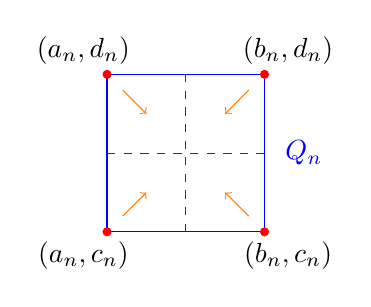
\begin{tikzpicture}
\draw[blue] (0,0) rectangle (2,2);
\node[blue] () at (2.5,1) {\(Q_n\)};
\draw[red, fill] (0,0) circle [radius=0.5mm];
\draw[red, fill] (2,0) circle [radius=0.5mm];
\draw[red, fill] (0,2) circle [radius=0.5mm];
\draw[red, fill] (2,2) circle [radius=0.5mm];
\node[] () at (-0.3,-0.3) {\((a_n,c_n)\)};
\node[] () at (2.3,-0.3) {\((b_n,c_n)\)};
\node[] () at (-0.3,2.3) {\((a_n,d_n)\)};
\node[] () at (2.3,2.3) {\((b_n,d_n)\)};
\draw[violet, dashed] (0,1) -- (2,1);
\draw[violet, dashed] (1,0) -- (1,2);
\draw[->, orange] (0.2,0.2) -- (0.5,0.5);
\draw[->, orange] (1.8,0.2) -- (1.5,0.5);
\draw[->, orange] (0.2,1.8) -- (0.5,1.5);
\draw[->, orange] (1.8,1.8) -- (1.5,1.5);
\end{tikzpicture}
\end{center}
No matter which quadrant \(Q_{n+1}\) is, the four corners must ``move'' in the
direction suggested by the \orc{orange} arrows (or do not ``move''). More
precisely, we have:
\begin{itemize}
\item \(\{a_n\}\) and \(\{c_n\}\) are increasing; and
\item \(\{b_n\}\) and \(\{d_n\}\) are decreasing.
\end{itemize}
Considering the initial large square \([-N,N]^{2}\), we can see that
\(\{a_n\}\) and \(\{c_n\}\) are bounded above, and the sequences \(\{b_n\}\)
and \(\{d_n\}\) are bounded below. Since the side lengths of the quadrants are
shrinking (by half each time), we can apply monotone convergence theorem to
argue that there exist \(x_0,y_0\in\R\) such that: 
\begin{itemize}
\item \(\{a_n\}\to x_0\), \(\{b_n\}\to x_0\); and
\item \(\{c_n\}\to y_0\), \(\{d_n\}\to y_0\).
\end{itemize}
\end{pf}

\textbf{Claim:} The point \(p=(x_0,y_0)\) is an accumulation point of \(S\).

\begin{pf}
It suffices to show that for any \(r>0\), \(B(p,r)\supseteq Q_n\) for some
\(n\in\N\), as this would then imply that \(B(p,r)\) contains infinitely many
points of \(S\), and thus \(p\) is an accumulation point of \(S\) by \Cref{prp:acc-pt-inf-set}.

Fix any \(r>0\). Since \(\{(a_n,c_n)\}\to p\), there exists \(M_1\in\N\) such
that
\[
d(p,(a_n,c_n))<\frac{r}{4}
\]
for any positive integer \(n\ge M_1\). Also, there exists \(M_2\in\N\) such that
the side length of \(Q_n\)
\[
\ell(Q_n)<\frac{r}{4}
\]
for any \(n\ge M_2\), as the side lengths are shrinking.

Take \(M=\max\{M_1,M_2\}\), and choose any \(n\ge M\).  We then have for any
\(q\in Q_n\),
\[
d(q,p)\le d(q,(a_n,c_n))+d((a_n,c_n),p)
\le \sqrt{2}\ell(Q_n)+\frac{r}{4}
\le \frac{\sqrt{2}}{4}r+\frac{r}{4}
=\frac{\sqrt{2}+1}{4}r
<r.
\]
So, \(Q_n\subseteq B(p,r)\) as desired.
\begin{center}
\begin{tikzpicture}
\draw[blue] (0,0) rectangle (2,2);
\node[blue] () at (2.5,1) {\(Q_n\)};
\draw[red, fill] (0,0) circle [radius=0.5mm];
\draw[red, fill] (2,0) circle [radius=0.5mm];
\draw[red, fill] (0,2) circle [radius=0.5mm];
\draw[red, fill] (2,2) circle [radius=0.5mm];
\node[] () at (-0.3,-0.3) {\((a_n,c_n)\)};
\draw[brown, fill] (0.5,0.7) circle [radius=0.5mm];
\node[] () at (0.7,1) {\(p\)};
\draw[pen colour=ForestGreen, very thick, decorate,decoration={calligraphic brace, amplitude=5pt, raise=0}] (0,0) -- (0.5,0.7)
node[left=0.3cm, midway]{\(<r/4\)};
\draw[pen colour=ForestGreen, very thick, decorate,decoration={mirror, calligraphic brace, amplitude=5pt, raise=0}] (0,0) -- (2,0)
node[below=0.2cm, midway]{\(<r/4\)};
\draw[brown, dashed] (0.5, 0.7) circle [radius=5cm];
\node[brown] () at (3,4) {\(B(p,r)\)};
\end{tikzpicture}
\end{center}
\end{pf}

The result then follows by this claim.
\end{pf}

\begin{note}
It is crucial that the metric \(d\) is Euclidean distance in this proof.
\end{note}

\item The next theorem is also a generalization to a theorem studied in
MATH2241. This time it generalizes \emph{nested interval theorem}, and it is
known as \emph{Cantor intersection theorem}. Boltzano-Weierstrass theorem in
needed in its proof below.
\begin{theorem}[Cantor intersection theorem]
\label{thm:cantor-intersection}
Every decreasing nest of closed and bounded nonempty subsets of \(\R^n\) has
nonempty intersection. Symbolically, if \(\{Q_k\}_{k=1}^{\infty}\) is a
sequence of non-empty closed subsets of \(\R^n\) satisfying
\begin{enumerate}
\item \(Q_{k+1}\subseteq Q_k\) for any \(k\in\N\), and
\item \(Q_1\) is bounded,
\end{enumerate}
then \(\displaystyle \bigcap_{k=1}^{\infty}Q_k\ne\varnothing\).
\end{theorem}
\begin{pf}
Assume to the contrary that 
\begin{equation}
\label{eq:cantor-int-contrary-assum}
\bigcap_{k=1}^{\infty}Q_k=\varnothing.
\end{equation}
Then consider the following.
\begin{enumerate}[label={(\arabic*)}]
\item Since \(Q_1\) is nonempty by assumption, there exists \(x_1\in Q_1\triangleq Q_{n_1}\). By
\Cref{eq:cantor-int-contrary-assum}, there exists \(n_2\in\N\) such that \(x_1\notin
Q_{n_2}\); Otherwise, the intersection would contain at least \(x_1\).
\item Since \(Q_{n_2}\) is nonempty, there exists \(x_2\in Q_{n_2}\).
By \Cref{eq:cantor-int-contrary-assum}, there exists \(n_3\in\N\) such that
\(x_2\notin Q_{n_3}\).
\item Since \(Q_{n_3}\) is nonempty, there exists \(x_3\in Q_{n_3}\).
By \Cref{eq:cantor-int-contrary-assum}, there exists \(n_4\in\N\) such that
\(x_3\notin Q_{n_4}\).
\item ...
\end{enumerate}
Continuing in this way, we would get a sequence \(\{x_i\}_{i=1}^{\infty}\) such
that \(x_i\notin Q_{n_i}\) for any \(i\in\N\).
\begin{center}
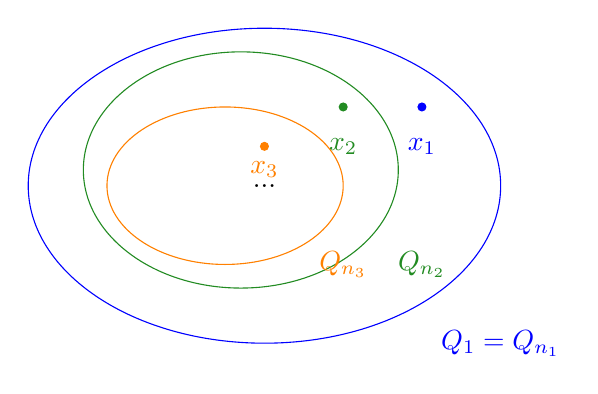
\begin{tikzpicture}
\draw[blue] (0,0) ellipse [x radius=3cm, y radius=2cm];
\node[blue] () at (3,-2) {\(Q_1=Q_{n_1}\)};
\draw[blue, fill] (2,1) circle [radius=0.5mm];
\node[blue] () at (2,0.5) {\(x_1\)};
\draw[ForestGreen] (-0.3,0.2) ellipse [x radius=2cm, y radius=1.5cm];
\node[ForestGreen] () at (2,-1) {\(Q_{n_2}\)};
\draw[ForestGreen, fill] (1,1) circle [radius=0.5mm];
\node[ForestGreen] () at (1,0.5) {\(x_2\)};
\draw[orange] (-0.5,0) ellipse [x radius=1.5cm, y radius=1cm];
\node[orange] () at (1,-1) {\(Q_{n_3}\)};
\draw[orange, fill] (0,0.5) circle [radius=0.5mm];
\node[orange] () at (0,0.2) {\(x_3\)};
\node[] () at (0,0) {...};
\end{tikzpicture}
\end{center}
By construction of the sequence \(\{x_i\}\), we have the following properties.
\begin{enumerate}
\item The set \(\{x_i:i\in\N\}\) is bounded, since \(Q_1\) is bounded.
\item The set \(\{x_i:i\in\N\}\) contains infinitely many elements since the
sequence contains distinct terms, i.e., \(x_{i}\ne x_{j}\) for any \(i\ne j\).
\end{enumerate}
Then, by Boltzano-Weierstrass theorem (\Cref{thm:boltzano-weierstrass}), the
set \(\{x_i:i\in\N\}\), being an infinite bounded subset of \(\R^n\), has an
accumulation point \(p\) in \(\R^n\). We then want to show that \(\displaystyle
p\in \bigcap_{k=1}^{\infty}Q_k\) to arrive at a contradiction.

Fix any \(k\in\N\). By assumption, \(Q_k\) is closed, so \(\overline{Q}_k=Q_k\).
Hence, it suffices to show that \(p\) is an adherent point of \(Q_k\), which
would then imply that \(p\in \overline{Q}_k=Q_k\). We shall prove this by
definition.

Fix any \(r>0\). Then we need to show that \(B(p,r)\cap Q_k\ne\varnothing\).
Since \(p\) is an accumulation point of the set \(\{x_i:i\in\N\}\), for any
\(r>0\) the open ball \(B(p,r)\) contains infinitely many points from
\(\{x_i:i\in\N\}\) by \Cref{prp:acc-pt-inf-set}. Hence, there exists \(m>k\)
such that \(B(p,r)\) contains \(x_m\). But we know that \(x_m\in Q_{n_m}\) also
by construction. So, we actually have
\[
x_m\in B(p,r)\cap Q_{n_m}\implies B(p,r)\cap Q_{n_m}\ne\varnothing.
\]
Note that \(n_m\ge m>k\), so \(Q_{n_m}\subseteq Q_k\) by assumption, implying
that
\[
B(p,r)\cap Q_{k}\ne\varnothing.
\]
Thus, \(p\in\overline{Q}_k=Q_k\). As \(k\in\N\) is arbitrary, it follows that
\(\displaystyle p\in\bigcap_{k=1}^{\infty}Q_k\), which contradicts
\Cref{eq:cantor-int-contrary-assum}.
\end{pf}

\item Using \emph{Cantor intersection theorem} and \emph{Lindel\"of's theorem},
we can prove the implication \(\text{(b)}\implies \text{(a)}\) under the metric
space \(\R^n\). This implication is also known as \emph{Heine-Borel theorem}.

\begin{theorem}[Heine-Borel theorem]
\label{thm:heine-borel}
Every closed and bounded subset of \(\R^n\) is compact.
\end{theorem}
\begin{pf}
Consider any closed and bounded set \(S\subseteq \R^n\). Let
\(\mathcal{U}=\{U_{\lambda}:\lambda\in\Lambda\}\) be any open cover of \(S\),
i.e.,
\[
\bigcup_{\lambda\in\Lambda}U_{\lambda}\supseteq S
\]
where \(U_{\lambda}\) is open (in \(\R^n\)) for any \(\lambda\in\Lambda\). To
show the compactness, we want to find a finite subcover of \(\mathcal{U}\).

We first use Lindel\"o{f}'s theorem (\Cref{thm:lindelof}). It suggests that
there exists a countable family \(\{U_k\}_{k=1}^{\infty}\) such that for any
\(k\in\N\), \(U_k=U_{\lambda}\) for some \(\lambda\in\Lambda\), and it satisfies
\[
\bigcup_{k=1}^{\infty}U_k=\bigcup_{\lambda\in\Lambda}U_{\lambda}\supseteq S
\]

Next, let \(\displaystyle Q_k=\bigcup_{i=1}^{k}U_i\), which is open since it is
an union of open sets. Then, we have
\[
\bigcup_{k=1}^{\infty}Q_k=\bigcup_{i=1}^{\infty}U_i\supseteq S.
\]
\textbf{Claim:} There exists \(N\in\N\) such that \(\displaystyle
Q_{N}=\bigcup_{i=1}^{N}U_i\supseteq S\) .

\begin{pf}
Assume to the contrary that for any \(k\in\N\), \(S\) contains some elements
not in \(Q_k\), i.e., \((X\setminus Q_{k})\cap S\ne\varnothing\). For any
\(k\in\N\), note that:
\begin{itemize}
\item \((X\setminus Q_k)\cap S\) is closed (in \(\R^n\)) since \(X\setminus
Q_k\) and \(S\) are both closed, so do their intersection.
\item \((X\setminus Q_k)\cap S\) is bounded since \(S\) is bounded.
\item \((X\setminus Q_{k+1})\subseteq (X\setminus Q_k)\).
\end{itemize}
Then, applying Cantor intersection theorem (\Cref{thm:cantor-intersection}),
\[
\bigcap_{k=1}^{\infty}[(X\setminus Q_k)\cap S]\ne\varnothing.
\]
But on the other hand, we have
\begin{align*}
\bigcap_{k=1}^{\infty}[(X\setminus Q_k)\cap S]
&=\bigcap_{k=1}^{\infty}[(X\cap S)\setminus (Q_k\cap S)]\\
&=\bigcap_{k=1}^{\infty}[S\setminus (Q_k\cap S)]\\
&=S\setminus \qty[\bigcup_{k=1}^{\infty}(Q_k\cap S)]\\
&=S\setminus \qty[\qty(\bigcup_{k=1}^{\infty}Q_k)\cap S]\\
&=S\setminus S&\text{(since \(\textstyle\bigcup_{k=1}^{\infty}Q_k\supseteq S\))}\\
&=\varnothing.
\end{align*}
Contradiction.
\end{pf}

By the claim, we know that \(\{U_1,\dotsc,U_N\}\) is a finite subcover of
\(\mathcal{U}\), as desired.
\end{pf}


\item Now, we are ready to prove the main result in
\Cref{subsect:compactness-rn} as follows.

\begin{theorem}
\label{thm:cpt-equiv-criteria-rn}
Let \(S\) be a subset of \(\R^n\). Then the following are equivalent.
\begin{enumerate}
\item \(S\) is compact.
\item \(S\) is closed and bounded.
\item \(S\) has the Boltzano-Weierstrass property.
\end{enumerate}
\end{theorem}
\begin{pf}
So far we have proved that \(\text{(a)}\iff\text{(b)}\)
(\Cref{thm:compact-imp-closed-bounded,thm:heine-borel}) and
\(\text{(a)}\implies \text{(c)}\) (\Cref{thm:cpt-bw-prop}). Hence, it
suffices to prove that \(\text{(c)}\implies \text{(b)}\).

First, assume that \(S\) has the Boltzano-Weierstrass property. We will first
prove the \underline{boundedness} of \(S\). Assume to the contrary that \(S\)
is not bounded (which implies that it is infinite). Then, for any \(k\in\N\) we
can pick \(x_k\in S\) such that \(x_k\ge k\). But then the infinite set
\(\{x_k:k\in\N\}\) cannot possibly have an accumulation point. For example,
every open ball with radius \(1/2\) cannot possibly contain infinitely many
\(x_n\)'s. Contradiction.

Next, we will prove the \underline{closedness} of \(S\). By
\Cref{prp:equiv-crit-closed}, it suffices to prove that \(\overline{S}=S\).  We
know that \(S\subseteq \overline{S}\) always, so it actually suffices to show
that \(\overline{S}\subseteq S\). By
\labelcref{it:closure-decompose-acc-isolate}, every point in \(\overline{S}\)
is either an accumulation point or isolated point of \(S\). Since isolated
point of \(S\) must belong to \(S\) by definition, it remains to show that
\emph{every accumulation point of \(S\) belongs to \(S\)}.

Let \(x\in\R^n\) be any accumulation point of \(S\). Then, for any \(k\in\N\),
setting the radius \(r=1/k\), there exists \(x_k\in B(x,1/k)\cap S\). Since each open
ball \(B(x,1/k)\) contains infinitely many points in \(S\), we can require the
\(x_n\)'s to be all distinct, i.e., \(x_k\ne x_m\) for any positive integers
\(n\ne m\). This then forms an infinite subset \(\{x_k:k\in\N\}\) of \(S\). By
the Boltzano-Weierstrass property of \(S\), the set \(\{x_k:k\in\N\}\) has an
accumulation point \(y\in S\).

\textbf{Claim:} We have \(x=y\in S\).

\begin{pf}
Assume to the contrary that \(x\ne y\). Then, let \(r_0=d(y,x)>0\). Consider
the open ball \(B(y,r_0/2)\). Since \(y\) is an accumulation point of
\(\{x_k:k\in\N\}\), \(B(y,r_0/2)\) contains infinitely many \(x_n\)'s by
\Cref{prp:acc-pt-inf-set}. Choose a large \(N\in\N\) such that \(1/N<r_0/2\).
Then, there exists \(k>N\) such that \(d(y,x_k)<r_0/2\). Also, for this \(k\),
we have \(d(x_k,x)<1/k<1/N\) as \(x_k\in B(x,1/k)\). Hence,
\[
d(y,x)\le d(x_k,x)+d(y,x_k)
<\frac{1}{N}+\frac{r_0}{2}
<\frac{r_0}{2}+\frac{r_0}{2}
=r_0,
\]
contradicting to the fact that \(r_0=d(y,x)\).
\end{pf}

By the claim, the arbitrarily chosen accumulation point \(x\) belongs to \(S\),
as desired.
\end{pf}
\end{enumerate}
